\documentclass{article}
\usepackage{amsmath}
\usepackage{natbib}
\usepackage[textwidth=5.8in, textheight=8in]{geometry}
\usepackage{lipsum}
\usepackage[mathscr]{eucal}
\usepackage{graphicx}

\newcommand{\T}{\frac{\theta}{2}}
\newcommand{\E}{\mathrm{E}}
\newcommand{\Var}{\mathrm{Var}}
\newcommand{\Cov}{\mathrm{Cov}}
\newcommand{\Pro}{\mathrm{P}}
\newcommand{\Kurt}{\mathrm{Kurt}}

\begin{document}

\section{Moment generating functions for the distribution of quantitative trait values}
\subsection{A generalized form}
\subsubsection{Stepping stone mutation model}
A basic question in quatitative genetics is what is the distribution of trait
values in a sample of individuals. In their investigation, \citet{Schraiber2015}
found a generating function for this distribution undes the standard neutral
coalescent model and a general stepping stone model of mutation. We wish to
extend this framework to additional populatio models. A first step is to show a
connection between the distribution of branch lengths on a genealogy and the
distribution of trait values in the sampled individuals. This should be useful
because the generating functions under various models of population structure
have already been investigated in some depth \citep{Lohse2011}.

Let $\mathbf{T}$ be a random vector containing the lengths of all possible
branches on a coalescent tree. For instance, if we had a three samples $a$, $b$,
and $c$, then $\mathbf{T}=\{T_a,T_b,T_c,T_{a,b},T_{a,c},T_{b,c}\}$. Let
$\mathcal{O}$ contain all possible configurations that coalescent branches can
subtend. For our example, $\mathcal{O}=\{(a),(b),(c),(a,b),(a,c),(b,c)\}$. Let
$\mathbf{Y}$ be a random vector containing the quantitative trait values in the
sampled individuals. For our example, $\mathbf{Y}=\{Y_a,Y_b,Y_c\}$. It is
important to note that these values indicate the change in the quantitative
trait since the value in the MRCA of the sample, not their actual values.

The moment generating function of $\mathbf{Y}$ is
\begin{equation}
  \varphi_{\mathbf{Y}}(\mathbf{k}) = E\left[ e^{\mathbf{k} \cdot \mathbf{Y}} \right] =
  \int e^{\mathbf{k} \cdot \mathbf{Y}} P(\mathbf{Y}=\mathbf{y}) d\mathbf{y},
\end{equation}
where $\mathbf{k}$ is a vector of dummy variables for each
sample. Although imperfect, this is the notation I will use for
writing integrals over probability distributions. Rewriting this
expression by conditioning on the genealogy we get
\begin{align}
  \varphi_{\mathbf{Y}}(\mathbf{k}) &= \int e^{\mathbf{k} \cdot \mathbf{Y}}
  \int P(\mathbf{Y}=\mathbf{y} | \mathbf{T}=\mathbf{t}) P(\mathbf{T}=\mathbf{t})
  d\mathbf{t} d\mathbf{y}\\
  &= \int \int e^{\mathbf{k} \cdot \mathbf{Y}} P(\mathbf{Y}=\mathbf{y} | \mathbf{T}=\mathbf{t}) d\mathbf{y}
  P(\mathbf{T}=\mathbf{t})
  d\mathbf{t}
\end{align}

We can write each $Y_i$ as a sum of the change in the trait value
occuring on each branch of the genealogy.
\begin{equation}
  Y_i = \sum_{\omega \in \mathcal{O}} Y_{i,\omega}
\end{equation}
Of course, many of these branches will not subtend $i$, so the change
along them is defined to be zero. The $Y_{i,\omega}$ are correlated
because the underlying branch lengths are correlated, but they are
conditionally independent given $\mathbf{T}$. This is due to the
assumption of a stepping stone mutation model and that mutations occur
as a poisson process along the branches. We can therefore factor $\int
e^{\mathbf{k} \cdot \mathbf{Y}} P(\mathbf{Y}=\mathbf{y}
|\mathbf{T}=\mathbf{t}) d\mathbf{y}$ into independent parts. We first write
\begin{equation}
  \mathbf{k} \cdot \mathbf{y} = \sum_{\omega \in \mathcal{O}}\left( \sum_{i \in \omega} k_iy_{i,\omega}\right)
\end{equation}
and
\begin{equation}
  P(\mathbf{Y}=\mathbf{y}|\mathbf{T}=\mathbf{t}) = \prod_{\omega \in \mathcal{O}}
  P(\mathbf{Y}_{\omega}=(y_{i,\omega})_{i \in \omega} | \mathbf{T}=\mathbf{t}).
\end{equation}
This yields
\begin{equation} \label{eq:factor}
  \int e^{\mathbf{k} \cdot \mathbf{Y}} P(\mathbf{Y}=\mathbf{y} |\mathbf{T}=\mathbf{t}) d\mathbf{y} =
  \prod_{\omega \in \mathcal{O}}\int \exp\left(\sum_{i \in \omega}k_iy_{i,\omega}\right)
  P(\mathbf{Y}_{\omega}=(y_{i,\omega})_{i \in \omega} | \mathbf{T}=\mathbf{t})d(y_{i,\omega})_{i \in \omega}.
\end{equation}

To move on we require two results. The first is that the change in a
trait value along some branch of length $t_\omega$ is a compound
Poisson process. The moment generating function for a compound Poisson
process over a time $t$ is $\exp\left(\lambda t (\psi(k)-1)\right)$.
Where $\lambda$ is the rate that events happen and $\psi$ is the
moment generating function for the distribution of mutation effects.
The second results is that the moment generating function for the
distribution of two completely correlated random variables $X_1$ and
$X_2$ that have the same distribution is $\varphi_{X_1}(k_1+k_2)$. Since
the trait change along a branch $t_{\omega}$ is the same for all
samples subtended by the branch, we can write the product terms in
equation \ref{eq:factor} as
\begin{equation}
  \exp\left( \frac{\theta}{2} t_{\omega} \left( \psi\left(\sum_{i \in \omega}k_{\omega}\right) -1 \right)\right).
\end{equation}
This gives
\begin{equation}
  \varphi_{\mathbf{Y}}(\mathbf{k}) = \prod_{\omega \in \mathcal{O}}
  \int \exp\left( \frac{\theta}{2} t_{\omega} \left( \psi\left(\sum_{a \in \omega}k_{a}\right) -1 \right)\right)
  P(\mathbf{T}=\mathbf{t})d\mathbf{t}.
\end{equation}
This is simply the moment generating function for the genealogy
$\mathbf{T}$ with $\frac{\theta}{2} \left( \psi(\sum_{i \in
  \omega}k_{\omega}) -1 \right)$ substituted for the dummy variable of
branch $T_{\omega}$. Or,
\begin{equation}
  \label{eq:sub}
  \varphi_{\mathbf{T}}(\mathbf{s})\Bigr|_{s_{\omega}=\frac{\theta}{2} \left( \psi\left(\sum_{a \in \omega}k_{a}\right) -1 \right)}
\end{equation}

%%% Local Variables:
%%% TeX-master: "notes.tex"
%%% End:

\subsubsection{House of cards mutation model}
The model used above is just one possible way in which mutations can affect
quantitative trait values. This model assumes that the contribution to the
phenotype of an individual from a locus $i$ is a linear combination of the
effects of mutations that have occured at the locus. Moreover, the phenotype of
an individual is a linear combination of all the mutations that have occured in
the genome of that individual. The big assumption is that each mutation at a
locus adds a random effect to the current effect of that locus. This model is
called the stepping stone model and was developed by \citet{Kimura1965}. An
alternative model is one in which each mutation causes the effect of that locus
to be drawn from some distribution, erasing the effects of all other mutations
that had occured at that locus in the past. This mutational model is called the
house of cards model and was developed by \citet{Kingman1978}. 

Here I derive a moment generating function for the house of cards model. This
turns out to have a more complicated form than the stepping stone model because
the effect of a mutation on an individual's phenotype depends on what other
mutations occur at that locus.

As before, the moment generating function is defined as 
\begin{equation}
  \varphi_{\mathbf{Y}}(\mathbf{k}) = E\left[ e^{\mathbf{k} \cdot \mathbf{Y}} \right] = 
  \int e^{\mathbf{k} \cdot \mathbf{Y}} P(\mathbf{Y}=\mathbf{y}) d\mathbf{y}.
\end{equation}
We employ the same tool of conditioning on the genealogy, $\mathbf{T}$, but we
additionally condition on the mutational configuration $\mathbf{M}$. The
mutational configuration is a vector whose entry $m_{\omega}$ is one if a
mutation occurs on branch $\omega$ and zero otherwise. This gives
\begin{align}
  \varphi_{\mathbf{Y}}(\mathbf{k}) &= \int e^{\mathbf{k} \cdot \mathbf{Y}}
  \int \int P(\mathbf{Y}=\mathbf{y} | \mathbf{M}=\mathbf{m}) 
  P(\mathbf{M}=\mathbf{m} | \mathbf{T}=\mathbf{t}) P(\mathbf{T}=\mathbf{t})
  d\mathbf{m} d\mathbf{t} d\mathbf{y}.\\
  &= \sum_{\mathbf{m}} \int e^{\mathbf{k} \cdot \mathbf{Y}} P(\mathbf{Y}=\mathbf{y} | \mathbf{M}=\mathbf{m}) d\mathbf{y} 
  \int P(\mathbf{M}=\mathbf{m}|\mathbf{T}=\mathbf{t}) P(\mathbf{T}=\mathbf{t})d\mathbf{t}
\end{align}
Of course, the phenotype values are conditionally independent of the genealogy
given the mutational configuration. The first integral is the difficult one
because it requires knowing the dependence structure of the phenotypic values
given the mutation configuration. Inidividual phenotypes will be zero if no
mutations occur, independent if mutations occur on different branches, and
completely correlated if mutations occur on the same branch. Additionally, only
the lowest level mutations count. By this we mean for each individual only the
mutations on the branch with the smallest number of descendents count. This can
be written succintly as
\begin{equation}
  \int e^{\mathbf{k} \cdot \mathbf{Y}} P(\mathbf{Y}=\mathbf{y} | \mathbf{M}=\mathbf{m}) d\mathbf{y} = 
  \prod_{\omega} \psi\left(\sum_{i \in \omega} k_i \mathscr{G}(i, \omega, \mathbf{m}) \right).
\end{equation}
Where 
\[
 \mathscr{G}(i,\omega,\mathbf{m}) = 
 \begin{cases}
   1 & \text{if }\omega\text{ is lowest level branch in }\mathbf{m}\text{ containing a mutation subtending }i\\
   0 & \text{otherwise}.
 \end{cases}
\]
The second integral can be written as
\begin{equation}
  \int \prod_\omega \left( m_\omega + (-1)^{m_\omega}e^{-\T t_\omega}\right)P(\mathbf{T}=\mathbf{t})d\mathbf{t}.
\end{equation}
This multiplies the probability that one or more mutations occur along a branch.
We can recognize that this will just be a sum of generating functions for the
genealogy evaluated at different $-\T \mathbf{m}$. It can therefore be written as 
\begin{equation}
  \sum_{\mathbf{m}'}(-1)^{\mathbf{m} \cdot \mathbf{m}'}\mathscr{K}(\mathbf{m}, \mathbf{m}')\varphi_T(-\T \mathbf{m}').
\end{equation}
Where
\[
\mathscr{K}(\mathbf{m}, \mathbf{m}') = 
\begin{cases}
  1 & \text{if } |\mathbf{m}| + \mathbf{m} \cdot \mathbf{m}' = sum(\mathbf{m}) + sum(\mathbf{m}')\\
  0 & \text{otherwise}.
\end{cases}
\]
This function returns one if $\mathbf{m}$ and $\mathbf{m}'$ contain none of the
same zero elements, and zero otherwise. 

The moment generating function overall can therefore be written as
\begin{equation}
  \sum_{\mathbf{m}}\left(\prod_{\omega} \psi\left(\sum_{i \in \omega} k_i 
\mathscr{G}(i, \omega, \mathbf{m}) \right) \right)
\left( \sum_{\mathbf{m}'}(-1)^{\mathbf{m} \cdot \mathbf{m}'}\mathscr{K}(\mathbf{m}, \mathbf{m}')
\varphi_T(-\T \mathbf{m}')\right).
\end{equation}
%%% Local Variables:
%%% TeX-master: "notes.tex"
%%% End:
\subsection{A central limit theorem}
Here we will show that the distribution of trait values is multivariate normal
regardless of the distribution of coalescent times. Recall that the moment
generating function for a general distribution of coalescence times is
\begin{equation}
  \varphi_T(\mathbf{s}) = \int \exp \left( \sum_{\omega \in \mathcal{O}} s_{\omega}t_{\omega} \right)
  P(\mathbf{T}=\mathbf{t})d\mathbf{t}.
\end{equation}
The Taylor series expansion of $\exp \left( s_{\omega}t_{\omega} \right)$ is
\begin{equation}
  1 + s_{\omega}t_{\omega} + \frac{s_{\omega}^2t_{\omega}^2}{2} + \ldots. \nonumber
\end{equation}
$\exp \left( \sum_{\omega \in \mathcal{O}} s_{\omega}t_{\omega} \right)$ is therefore
\begin{equation}
  1 + \sum_{\omega \in \mathcal{O}} s_{\omega}t_{\omega} +
  \sum_{\omega_1 \neq \omega_2} s_{\omega_1}t_{\omega_1}s_{\omega_2}t_{\omega_2} + 
  \sum_{\omega \in \mathcal{O}} \frac{s_{\omega}^2t_{\omega}^2}{2} + \ldots. \nonumber
\end{equation}
This of course means that
\begin{equation}
  \label{eq:mgf_L}
  \left(\int \exp \left( \sum_{\omega \in \mathcal{O}} s_{\omega}t_{\omega}
  \right)P(\mathbf{T}=\mathbf{t})d\mathbf{t}\right)^L = \left(1 + \sum_{\omega \in \mathcal{O}}
  s_{\omega}E[t_{\omega}] + \sum_{\omega_1 \neq \omega_2}
  s_{\omega_1}s_{\omega_2}E[t_{\omega_2}t_{\omega_1}] + \sum_{\omega \in
    \mathcal{O}} \frac{s_{\omega}^2E[t_{\omega}^2]}{2} + \ldots\right)^L. 
\end{equation}
Based on equation \ref{eq:sub} we can get the moment generating function for the
trait values by making the substitution $s_{\omega}\to \frac{\theta}{2} \left(
\psi\left(\sum_{a \in \omega}k_{a}\right) -1 \right)$. We will also take the
Taylor series of the moment generating function of the mutational distribution.
Noting that $\frac{d^n}{dk^n}\varphi_X(k)\Bigr|_{k=0} = E[X^n]$, if we let $m_1$
be the mean and $m_2$ be the second moment of the mutational distribution, then
\begin{equation}
  \psi\left( \sum_{a \in \omega} k_a \right) = 1 + m_1 \left( \sum_{a \in \omega}
  k_a\right) + m_2/2\left( \sum_{a \in \omega} k_a\right)^2 + \ldots.
  \nonumber
\end{equation}
Substituting this into equation \ref{eq:mgf_L} we get
\begin{align}
  \biggl( 1 &+ \frac{\theta}{2} \sum_{\omega \in \mathcal{O}} E[t_{\omega}]\left( m_1 \left(
  \sum_{a \in \omega} k_a \right) + \frac{m_2}{2} \left( \sum_{a \in \omega}
  k_a\right)^2 + \ldots \right) \\
  &+ \sum_{\omega_1 \neq \omega_2} \T\left( m_1 \sum_{a \in \omega_1} k_a + \ldots \right)
  \T \left( m_1 \sum_{b \in \omega_2} k_b + \ldots \right)
  E[t_{\omega_1\omega_2}] \\
  &+ \sum_{\omega \in \mathcal{O}} \left(\T\right)^2\left(m_1 \sum_{a \in \omega} k_a +
  \ldots \right)^2 E[t^2_{\omega}] \biggr)^L.
\end{align}
Now if we take the limit such that $L\T m_1 \to \mu$ and $L\T m_2\to \sigma^2$
as $L \to \infty$ we get
\begin{equation}
  \exp \left( \frac{\theta}{2} \sum_{\omega \in \mathcal{O}}E[t_{\omega}] \left( \mu \left(
  \sum_{a \in \omega} k_a\right) + \frac{\sigma^2}{2}\left( \sum_{a \in \omega}
  k_a\right)^2\right)\right),
\end{equation}
providing that the product of $L$ and moments of the mutational distribution
higher than two go to zero. This also requires that the limit of $L(\T)^2m_1$
goes to zero as the number of sites goes to infinity. $\mu$ can be interpreted
as the rate of change in the mean trait value per generation per genome due to
mutational pressure. $\sigma^2$ can be interpreted as the rate of accumulation
of variance in trait values per generation per genome. Ignoring terms with
$(\T)^2$ is equivalent to the assumption that mutation rates are low enough that
only one mutation per locus occurs. It is clear from inspection that this is the
moment generating function for a multivariate normal distribution where the
expected trait value is $E[T_{MRCA}] \mu$, the variance in a trait value is
$E[T_{MRCA}]\sigma^2$, and the covariance in trait values is
$(T_{MRCA}-E[\tau_{1,2}]) \sigma^2$. This covariance is proprtional to the
expected amount of shared branch length before the most recent common ancestor
of the sample.
%%% Local Variables:
%%% TeX-master: "notes.tex"
%%% End:

\subsection{Calculation of moments}
\subsubsection{Low mutation rate approximation}
The main utility of moment generating functions is to calculate moments. We
showed how the distribution of trait values converges to a normal distribution
when there are a large number of sites with small effect per mutation relative
to the rate of mutation. In order to see how much deviation there is from this
normal model we can calculate moments and compare them to the moments of the
multivariate normal distribution.

At first we will do this using the same low mutation rate approximation that was
used for the normal limit. The moment generation function of the trait values can 
be approximated as
\begin{equation}
  \label{eq:mgf_approx_1}
  \varphi_{\mathbf{Y}}(\mathbf{k}) \approx \left[ 1 + \sum_{\omega \in \mathcal{O}}
    E[t_\omega] \T \left( \Phi\left( \sum_{a \in \omega} k_a\right) -1 \right) \right]^L.
\end{equation}
This expression ignores any terms of the genealogy moment generation function
shown in equation \ref{eq:mgf_L} above order one. These terms are not written
because they contain products of mutation rates and coalescent times of order
two and greater. Removing these terms means that equation \ref{eq:mgf_approx_1}
is free of terms giving the expectations of products such as $E[\T t_{\omega_1}
  \T t_{\omega_2}]$, but it still contains products of expectations like $E[\T
  t_{\omega_1}]E[\T t_{\omega_2}]$. Both correspond to the instance where
multiple mutations occurs at a single locus. Such terms can be eliminated
entirely if substitute the Taylor series of the moment generating function of
the mutational distribution into equation \ref{eq:mgf_approx_1}. This gives
\begin{equation}
  \label{eq:mgf_approx_2}
  \varphi_{\mathbf{Y}}(\mathbf{k}) \approx
  1 + \T L \sum_{\omega \in \mathcal{O}} E[t_\omega]
  \left( \sum_{n=1}^\infty \frac{m_n}{n!} ( \sum_{a \in \omega}k_a)^n\right).
\end{equation}
Taking derivatives of equation \ref{eq:mgf_approx_2} and setting $\mathbf{k}$
equal to zero allows easy calculation of any moment of the trait value
distribution. For instance, the moment $E[y_a^i y_b^j y_c^k]$ is
\begin{equation}
  \T L \frac{m_{i+j+k}}{i!j!k!} \sum_{\omega : a,b,c \in \omega} E[t_\omega].
\end{equation}
This has the property that any moment is proportional to the expected shared
branch length. 

\subsubsection{The second moment and variance}
We can use the low mutation rate approximation to the moment generating function
(equation \ref{eq:mgf_approx_1}) to calculate moments of the distribution of
trait vales. We'll start by calculating the first and second moments and compare
these to the mean and variance of the normal distribution. We start, as we did
in deriving the normal distribution, by substituting the Taylor series of the
mutational mgf.
\begin{equation}
  \label{eq:mgf_approx_sub}
  \varphi_{\mathbf{Y}}(\mathbf{k}) \approx \left[ 1 + \sum_{\omega \in \mathcal{O}}
    E[t_\omega] \T \left( m_1 \sum_{a \in \omega} k_a +
    \frac{m_2}{2!}\left( \sum_{a \in \omega} k_a\right)^2 +
    \frac{m_3}{3!}\left( \sum_{a \in \omega} k_a\right)^3 +
    \frac{m_4}{4!}\left( \sum_{a \in \omega} k_a\right)^4 \ldots \right) \right]^L
\end{equation}
We can expand this out using multinomial coefficients to get
\begin{align}
  \label{eq:mgf_approx_expand}
  \varphi_{\mathbf{Y}}(\mathbf{k}) &\approx 1 +
  L\T \sum_{\omega \in \mathcal{O}} E[t_{\omega}]\left( m_1 \sum_{a \in \omega} k_a +
  \frac{m_2}{2}\left( \sum_{a \in \omega} k_a\right)^2 + \ldots \right) \nonumber \\
  &+ \frac{L(L-1)}{2} \left(\T\right)^2 \sum_{\omega \in \mathcal{O}} E[t_{\omega}]^2
  \left( m_1 \sum_{a \in \omega} k_a +
  \frac{m_2}{2}\left( \sum_{a \in \omega} k_a\right)^2 + \ldots \right)^2 \nonumber \\
  &+ L(L-1)\left(\T\right)^2\sum_{\omega_1, \omega_2 \in \mathcal{O}}E[t_{\omega_1}]E[t_{\omega_2}]
  \left( m_1 \sum_{a \in \omega_1} k_a + \ldots \right)
  \left( m_1 \sum_{a \in \omega_2} k_a + \ldots \right) + \ldots.
\end{align}
The first coefficient is $\binom{L}{L-1,1,\mathbf{0}}$, the second is
$\binom{L}{L-2,2,\mathbf{0}}$, and the third is $\binom{L}{L-2,1,1,\mathbf{0}}$.
This is probably not the best way to think about the combinatorics, but it will
do for now. To calculate the moments of this distribution one takes the partial
derivatives of the mgf and sets the dummy variables to zero.
\begin{equation}
  \label{eq:deriv}
  E[Y_1^{r_1}\ldots Y_n^{r_n}] = \frac{\partial^{r_1 + \ldots + r_n}}{\partial k_1^{r_1} \ldots \partial k_n^{r_n}}
  \varphi_{\mathbf{Y}}(\mathbf{k})\Bigr|_{\mathbf{k}=0}
\end{equation}
Using this to calculate the first moment of the trait distribution we get
\begin{equation}
  \label{eq:mom1}
  E[Y_a] \approx L\T m_1 \sum_{\omega : a \in \omega} E[t_\omega].
\end{equation}
The second moment is more complicated because there are $k_a^2$ terms in all
three lines of equation \ref{eq:mgf_approx_expand}.
\begin{align}
  E[Y_a^2] &\approx L\T m_2 \sum_{\omega : a \in \omega} E[t_\omega] \nonumber \\
  &+ \frac{L(L-1)}{2} \left(\T \right)^2 m_1^2 \sum_{\omega : a \in \omega} 2 E[t_\omega]^2 \nonumber \\
  &+ L(L-1) \left(\T \right)^2 m_1^2 \sum_{\omega_1 , \omega_2: a \in \omega_1 , \omega_2} 2 E[t_{\omega_1}]E[t_{\omega_2}]
\end{align}
Terms with $(\T)^2$ are kept because they also include a second order term of
$L$ in front of them. We can now calculated the variance using $Var[Y]=E[Y^2] -
E[Y]^2$. The squared first moment can be written as
\begin{align}
  \left(L\T m_1 \sum_{\omega : a \in \omega} E[t_\omega] \right)^2 &=
  L^2\left(\T\right)^2 m_1^2 \sum_{\omega : a \in \omega} E[t_\omega]^2 \nonumber \\
  &+ L^2\left(\T\right)^2 m_1^2 \sum_{\omega_1 , \omega_2: a \in \omega_1 , \omega_2} E[t_{\omega_1}]E[t_{\omega_2}].
\end{align}
Subtracting this from the second moment gives
\begin{align}
  \label{eq:var}
  Var[Y_a] &\approx L\T m_2 \sum_{\omega : a \in \omega} E[t_\omega] \nonumber \\
  &- L \left(\T\right)^2 m_1^2 \sum_{\omega : a \in \omega}E[t_\omega]^2 \nonumber \\
  &-  2L \left(\T\right)^2 m_1^2 \sum_{\omega_1 , \omega_2: a \in \omega_1 , \omega_2} E[t_{\omega_1}]E[t_{\omega_2}] \nonumber \\
  &= L\T m_2 \sum_{\omega : a \in \omega} E[t_\omega] -
  L\left( \T m_1 \sum_{\omega : a \in \omega} E[t_\omega] \right)^2 \nonumber \\
  &= L\T m_2 E[t_{MRCA}] - L\left( \T m_1 E[T_{MRCA}] \right)^2 \\
  &\approx L\T m_2 E[t_{MRCA}]  \nonumber
\end{align}
The $(\T)^2$ terms are no only first order in $L$ so they can be ignored. This
is the same variance as in the normal distribution because the limit takes care
of these terms automatically.
%%% Local Variables:
%%% TeX-master: "notes.tex"
%%% End:

\subsubsection{The fourth moment}
Due to the large number of terms I only derive the fourth moment of the trait
value distribution for the case when the mean mutational effect is zero. Having
the mean equal to zero is also helpful when comparing against a normal
distribution because higher order moments of the normal distribution are easy to
calculate when the mean is zero. The terms of \eqref{eq:mgf_approx_sub} that
will appear in the fourth moment after we apply \eqref{eq:deriv} are
\begin{equation*}
  L \left(\T\right) \frac{m_4}{24}
  \sum_{\omega:a\in \omega} E[t_\omega] \left(\sum_{a \in \omega} k_a\right)^4
\end{equation*}
for the fourth moment along one branch,
\begin{equation*}
  \binom{L}{L-2,2,\mathbf{0}}\left(\T\right)^2\left(\frac{m_2}{2}\right)^2
  24 \sum_{\omega:a\in \omega} E[t_\omega]^2 \left(\sum_{a \in \omega} k_a\right)^4
\end{equation*}
for the second moment of the same branch chosen twice, and
\begin{equation*}
  \binom{L}{L-2,1,1,\mathbf{0}}\left(\T\right)^2\left(\frac{m_2}{2}\right)^2
  24 \sum_{\omega_1 , \omega_2: a \in \omega_1 , \omega_2} E[t_{\omega_1}]E[t_{\omega_2}]
  \left(\sum_{a \in \omega_1} k_a\right)^2\left(\sum_{a \in \omega_2} k_a\right)^2
\end{equation*}
for the second moments on two different branches. Taking the fourth derivatives
of these in terms of the desired branch we get
\begin{align}
  \label{eq:mom4}
  E[Y_a^4] &= L\T m_4 E[T_{MRCA}] \nonumber \\
  &+ \frac{L(L-1)}{2} \left(\T\right)^2\left( \frac{m_2}{2} \right)^2
  24 \sum_{\omega:a\in \omega} E[t_\omega]^2 \nonumber \\
  &+ L(L-1) \left(\T\right)^2\left( \frac{m_2}{2} \right)^2
  24 \sum_{\omega_1 , \omega_2: a \in \omega_1 , \omega_2} E[t_{\omega_1}]E[t_{\omega_2}] \nonumber \\
  &= L\T m_4 E[T_{MRCA}] +
  3L(L-1)\left( \T m_2 \sum_{\omega:a\in \omega} E[t_\omega] \right)^2x \nonumber \\
  &= L\T m_4 E[T_{MRCA}] +
  3L(L-1)\left( \T m_2 E[T_{MRCA}] \right)^2 \\
  &\approx L\T m_4 E[T_{MRCA}] +
  3\left(L \T m_2 E[T_{MRCA}] \right)^2 \nonumber 
\end{align}
%%% Local Variables:
%%% TeX-master: "notes.tex"
%%% End:

\subsubsection{Kurtosis}
Since we know that the variance in trait values is very close under the low
mutation rate model as in the normal limit, we might next compare kurtosis which
provides a measure of the tailedness of the distribution. The kurtosis is
defined as
\begin{equation}
  Kurt[X]=\frac{E[(X-E[X])^4]}{(E[(X-E[X])^4)^2}.
\end{equation}
This is the fourth central moment divided by the variance. For ease of
calculation, we'll examine this in the case where the mean mutation effect (and
therefore trait value) is zero. If we plug \eqref{eq:var} and \eqref{eq:mom4}
into the expression for the kurtosis we get
\begin{align}
  \label{eq:kurtosis_single}
  Kurt[Y_a] &= \frac{L\T m_4 E[T_{MRCA}]}{\left(L\T m_2 E[T_{MRCA}]\right)^2} +
  \frac{3L(L-1)\left( \T m_2  E[T_{MRCA}]\right)^2}{\left(L\T m_2 E[T_{MRCA}]\right)^2} \nonumber \\
  &= \frac{m_4}{L\T m_2^2E[T_{MRCA}]} + \frac{3(L^2-L)}{L^2} \nonumber \\
  &= \frac{Kurt[M]}{L\T E[T_{MRCA}]} + 3\left( 1 - \frac{1}{L} \right).
\end{align}
What does this mean? The normal approximation will have a kurtosis of $3$, so
having a finite number of loci will act to decrease the kurtosis of the trait
distribution. However, it seems this decrease will only be very slight. The term
on the left shows that the kurtosis is increased by the ratio of the kurtosis of
the mutational distribution relative to the expected number of segregating sites
affecting the trait.
%%% Local Variables:
%%% TeX-master: "notes.tex"
%%% End:

\subsubsection{Cokurtosis}
Similarly to kurtosis, we can calculate another fourth order moment called the
cokurtosis which measures the propensity of extreme values to occur together in
the joint distribution. The cokurtosis is defined as
\begin{equation}
  \label{eq:cokurtosis_def}
  Cokurt(X,X,Y,Y)=\frac{E[(X-E[X])^2(Y-E[Y])^2]}{\sigma_X^2\sigma_Y^2}.
\end{equation}
We will only look at the balanced version of this for now. As with covariance,
the kurtosis of a random variable is its cokurtosis with itself. Courtesies may
be of interest residual signal of individual genealogies may cause individual to
share extreme trait values due to shared ancestry. We calculate the cokurtosis
by first calculating $E[Y_a^2Y_b^2]$ in the same way as was done for the
kurtosis by considering different terms of \eqref{eq:mgf_approx_sub}. One is the
fourth moment term for branches containing both $a$ and $b$:
\begin{equation*}
  L \T \frac{m_4}{4!} \sum_{\omega : a, b \in \omega} E[t_\omega] \left( \sum_{d \in \omega} k_d \right)^4.
\end{equation*}
Another is the second moment terms for pairs of branches both containing $a$ and $b$:
\begin{equation*}
  \frac{L(L-1}{2} \left( \sum_{\omega : a, b \in \omega}
  E[t_\omega] \T \frac{m_2}{2} \left( \sum_{d \in \omega} k_d \right)^2right).
\end{equation*}
Let $\Omega_{a/b}$ be the set of branches containing $a$ but not $b$ and
$\Omega_{a+b}$ be the set of branches containing both $a$ and $b$. We also need
to consider terms from $\Omega_{a/b}\times\Omega_{b}$ and
$\Omega_{b/a}\times\Omega_{a}$. These are
\begin{equation}
  L(L-1) \left( \sum_{\omega_1 \in \Omega_{a/b}} E[t_{\omega_1}] \T \frac{m_2}{2}
  \left( \sum_{d_1 \in \omega} k_{d_1} \right)^2 \right)
  \left( \sum_{\omega_2 \in \Omega_{b}} E[t_{\omega_2}] \T \frac{m_2}{2}
  \left( \sum_{d_2 \in \omega} k_{d_2} \right)^2 \right),
\end{equation}
and it's equivalent. Taking the appropriate derivatives we get
\begin{align*}
  E[Y_a^2Y_b^2] &= L \T m_4 \sum_{\omega \in \Omega_{a+b}} E[t_\omega] \\
  &+ 3L(L-1) \left( \sum_{\omega \in \Omega_{a+b}} \T m_2 E[t_\omega] \right)^2\\
  &+ L(L-1) \left( \sum_{\omega_1 \in \Omega_{a/b}} E[t_{\omega_1}] \T m_2  \right)
  \left( \sum_{\omega_2 \in \Omega_{b}} E[t_{\omega_2}] \T m_2 \right)\\
  &+ L(L-1) \left( \sum_{\omega_1 \in \Omega_{b/a}} E[t_{\omega_1}] \T m_2  \right)
  \left( \sum_{\omega_2 \in \Omega_{a}} E[t_{\omega_2}] \T m_2 \right)
\end{align*}
One way to simplify this is to notice that the last two lines almost sum over
$\Omega_a\times\Omega_b$ except that they are missing the product over terms
where both branches contain both $a$ and $b$. If we subtract one of the three
terms from the second line and add it here we get
\begin{align*}
  E[Y_a^2Y_b^2] &= L \T m_4 \sum_{\omega \in \Omega_{a+b}} E[t_\omega] \\
  &+ 2L(L-1) \left( \sum_{\omega \in \Omega_{a+b}} \T m_2 E[t_\omega] \right)^2\\
  &+ L(L-1) \left( \sum_{\omega_1 \in \Omega_{a}} E[t_{\omega_1}] \T m_2  \right)
  \left( \sum_{\omega_2 \in \Omega_{b}} E[t_{\omega_2}] \T m_2 \right),
\end{align*}
which can be rewritten as
\begin{equation}
  \label{eq:cross4}
  E[Y_a^2Y_b^2] = L \T m_4 E[\tau_{a+b}]+2L(L-1) \left(\T m_2 E[\tau_{a+b}]\right)^2
  + L(L-1) \left( \T m_2 E[\tau_a]\right)\left( \T m_2 E[\tau_b]\right).
\end{equation}
Since $E[\tau_a]$ is the expected length of branches in the entire genealogy
containing $a$, this is also the same as $E[T_{MRCA}]$.
%%% Local Variables:
%%% TeX-master: "notes.tex"
%%% End:

\subsubsection{Additional moments}
We also calculate here some additional moments that have less clear
interpretations but are useful later on when calculating the expected population
kurtosis. The first of these is $E[Y_a^3Y_b]$. The terms of
\eqref{eq:mgf_approx_sub} that will appear in this are
\begin{equation*}
  L \left(\T\right) \frac{m_4}{24} 4 k_a^3k_b \sum_{\omega:a,b \in \omega} E[t_\omega]
\end{equation*}
and
\begin{equation*}
  L(L-1)\left(\T \frac{m_2}{2}\right)^2 k_a^2 \times 2k_ak_b
  \left( \sum_{\omega:a,b \in \omega} E[t_\omega] \right) \left( \sum_{\omega: a \in \omega} E[t_\omega] \right).
\end{equation*}
This ultimately gives
\begin{equation}
  \label{eq:m31}
  E[Y_a^3Y_b] = L \T m_4 E[\tau_{a+b}] + 3L(L-1) \left(\T m_2\right)^2 E[T_{MRCA}]E[\tau_{a+b}].
\end{equation}
The next fourth moment of interest is $E[Y_a^2Y_bY_c]$. The terms of
\eqref{eq:mgf_approx_sub} are
\begin{equation*}
  L \T \frac{m_4}{24} 12k_a^2k_bk_c \sum_{\omega: a,b,c \in \omega} E[t_\omega],
\end{equation*}
\begin{equation*}
  L(L-1) \left(\T \frac{m_2}{2}\right)^2 k_a^2 \times 2k_bk_c
  \left( \sum_{\omega: a \in \omega} E[t_\omega] \right)\left( \sum_{\omega: a,b \in \omega} E[t_\omega] \right),
\end{equation*}
and 
\begin{equation*}
  L(L-1) \left(\T \frac{m_2}{2}\right)^2 2k_ak_b \times 2k_ak_c \left( \sum_{\omega: a,b \in \omega} E[t_\omega] \right)
  \left( \sum_{\omega: a,c \in \omega} E[t_\omega] \right).
\end{equation*}
Taking the appropriate derivatives of these gives
\begin{equation}
  \label{eq:m211}
  L \T m_4 E[\tau_{a+b+c}] + L(L-1)\left(\T m_2\right)^2E[T_{MRCA}]E[\tau_{b+c}] +
  2L(L-1) \left(\T m_2\right)^2E[\tau_{a+b}]E[\tau_{a+c}].
\end{equation}
Individuals in the population are exchangeable as long as it is not structured.
The pairwise expected shared branch lengths are in that case all equal and we
can write \eqref{eq:m211} as
\begin{equation}
  \label{eq:m211s}
  L \T m_4 E[\tau_{a+b+c}] + L(L-1)\left(\T m_2\right)^2E[T_{MRCA}]E[\tau_{a+b}] +
  2L(L-1) \left(\T m_2\right)^2E[\tau_{a+b}]^2.
\end{equation}
Where $\tau_{a+b}$ just refers to the expected shared branch length of any two
individuals in the population. The final moment we'll look at is
$E[Y_aY_bY_cY_d]$ which has relevant terms
%% The set of branches containing all individuals
\begin{equation*}
  L \T \frac{m_4}{24} 24k_ak_bk_ck_d \sum_{\omega: a,b,c,d \in \omega} E[t_\omega],
\end{equation*}
%% Cross set of a-b branches and c-d branches
\begin{equation*}
  L(L-1) \left(\T \frac{m_2}{2}\right)^2 2k_ak_b \times 2k_ck_d \left( \sum_{\omega: a,b \in \omega} E[t_\omega] \right)
  \left( \sum_{\omega: c,d \in \omega} E[t_\omega] \right),
\end{equation*}
%% Cross set of a-c branches and b-d branches
\begin{equation*}
  L(L-1) \left(\T \frac{m_2}{2}\right)^2 2k_ak_c \times 2k_bk_d \left( \sum_{\omega: a,c \in \omega} E[t_\omega] \right)
  \left( \sum_{\omega: b,d \in \omega} E[t_\omega] \right),
\end{equation*}
and
%% cross set of a-d branches and b-c branches
\begin{equation*}
  L(L-1) \left(\T \frac{m_2}{2}\right)^2 2k_ak_d \times 2k_bk_c \left( \sum_{\omega: a,d \in \omega} E[t_\omega] \right)
  \left( \sum_{\omega: b,c \in \omega} E[t_\omega] \right).
\end{equation*}
When the appropriate fourth order partial derivatives are taken of this we get
\begin{align*}
  L \T m_4 E[\tau_{a+b+c+d}] \\
  + L(L-1)\left(\T m_2\right)^2E[\tau_{a+b}]E[\tau_{c+d}] \\
  + L(L-1)\left(\T m_2\right)^2E[\tau_{a+c}]E[\tau_{b+d}] \\
  + L(L-1)\left(\T m_2\right)^2E[\tau_{a+d}]E[\tau_{b+c}].
\end{align*}
We can again simplify this expression for populations with exchangeable
individuals. This gives
\begin{equation}
  L \T m_4 E[\tau_{a+b+c+d}] \\
  + 3L(L-1)\left(\T m_2\right)^2E[\tau_{a+b}]^2.
\end{equation}
%%% Local Variables:
%%% mode: latex
%%% TeX-master: "notes.tex"
%%% End: 

\subsubsection{Comparison to normal distribution}
The Isserlis theorem states that the moments of a multivariate normal random
vector with mean zero is given by
\begin{equation}
  E[X_1X_2 \ldots X_n] = \sum \prod E[X_iX_j].
\end{equation}
The sum is over all possible ways of dividing the $n$ variables up into pairs,
and the product is over all pairwise expectations in that partition.
%%% Local Variables:
%%% TeX-master: "notes.tex"
%%% End:

\subsubsection{General moments}
Unfortunately, it does not seem possible to write down a simple solution to
\eqref{eq:deriv} that would provide and expression for an arbitrary moment of
the distribution of trait values. For an order $n$ term one would need to sum
over all orders of expected branch length terms that would appear in the
expansion of \eqref{eq:mgf_approx_sub}. For each order of branch lengths one
would need to sum over all possible sets of branch lengths and moments for those
branch lengths such that the desired product of dummy variables raised to the
correct powers could be produced. Furthermore, one would need to calculate the
coefficient for this product of dummy variables.

The one positive aspect about calculating general moments under the low mutation
rate approximation is that they only depend on the expected branch lengths.

%%% Local Variables:
%%% TeX-master: "notes.tex"
%%% End:

\subsection{Population moments}


%%% Local Variables: 
%%% mode: latex
%%% TeX-master: "notes.tex"
%%% End: 
\subsubsection{Population variance}
The expected variance of breeding values in the population, and what in this
model would be considered the genetic variance is

\begin{equation}
  \label{eq:popvar}
  E[V_g] = E\left[ \frac{1}{N}\sum \left( Y_i - \frac{\sum Y_j}{N} \right)^2\right].
\end{equation}

By assuming that all the individuals in the sample are exchangeable, we can
expand the inside to get

\begin{align*}
  E\left[ \left(  Y_i - \frac{\sum Y_j}{N} \right)^2 \right] &= 
                                                             E\left[ Y_i^2 - 2Y_i\frac{\sum Y_j}{N} + \left( \frac{\sum Y_j}{N} \right)^2 \right] \\
                                                           &= E[Y_i^2] - \frac{2}{N} E[Y_i^2] - 
                                                             \frac{2(N-1)}{N} E[Y_iY_j] + \frac{1}{N} E[Y_i^2] + 
                                                             \frac{N-1}{N} E[Y_iY_j] \\
                                                           &= \frac{N-1}{N} \left( E[Y_i^2] - E[Y_iY_j]\right).
\end{align*}

Thus when $N$ is even moderately large

\begin{equation}
  E[V_g] = E[Y_i^2] - E[Y_iY_j].
\end{equation}

When $m_1=0$, $E[Y_i^2] \approx L \T m_2 E[T_{MRCA}]$ and
$E[Y_iY_j] \approx L \T m_2 ( E[T_{MRCA}] - E[\tau_{i,j}])$. The expected
genetic variance in the population is then proportional to the expected pairwise
coalescent time as we would expect.
%%% Local Variables: 
%%% mode: latex
%%% TeX-master: "notes.tex"
%%% End: 

\subsubsection{Variance of population variance}
The variance of the population variance over evoultionary realizations is
another useful quantity. In the infinitesimal limit for a sufficiently large
population, the variance of the variance will be negligable relative to the
variance itself. That is, the coefficient of variation of the variance will
approach zero. Here I will derive the variance of the variance, from which one
could compute the coefficient of variation.

\begin{align}
  \label{eq:popvarvar}
  \Var[V_g] &= \Var\left[ \frac{1}{N}\sum \left( Y_i - \frac{\sum Y_j}{N} \right)^2\right] \nonumber \\
            &= \frac{1}{N^2}\left( \sum \Var[(Y_i - \frac{\sum Y_j}{N})^2] + 2 \sum_{i \neq j} 
              \Cov[(Y_i - \frac{\sum Y_k}{N})^2, (Y_j - \frac{\sum Y_k}{N})^2]\right).
\end{align}
The first term can be ignored if the population size is large. The second term
is determined by the covariance in the squared deviations from the mean. The
covariance can be calculated by considering its individual parts. 

\begin{align*}
  &\Cov[Y_i^2, Y_j^2] \approx -2\Cov[Y_i^2,Y_j^2] \nonumber \\
  &\Cov[Y_i^2, -2Y_j \frac{\sum Y_k}{N}] \approx -2\Cov[Y_i^2,Y_jY_k] \nonumber \\
  &\Cov[Y_i^2, \left(\frac{\sum Y_k}{N}\right)^2] \approx \Cov[Y_i^2,Y_jY_k] \nonumber \\
  &\Cov[-2Y_i\left(\frac{\sum Y_k}{N}\right), Y_j^2] \approx -2\Cov[Y_i^2,Y_jY_k] \nonumber \\
  &\Cov[-2Y_i\left(\frac{\sum Y_k}{N}\right),-2Y_j\left(\frac{\sum Y_k}{N}\right)] 
  \approx 4\Cov[Y_iY_j,Y_kY_l] \nonumber \\
  &\Cov[-2Y_i\left(\frac{\sum Y_k}{N}\right), \left(\frac{\sum Y_k}{N}\right)] 
  \approx -2\Cov[Y_iY_j,Y_kY_l] \nonumber \\
  &\Cov[\left(\frac{\sum Y_k}{N}\right)^2, Y_j^2] 
  \approx \Cov[Y_j^2,Y_iY_k] \nonumber \\
  &\Cov[\left(\frac{\sum Y_k}{N}\right)^2,-2Y_j\left(\frac{\sum Y_k}{N}\right)] 
  \approx -2\Cov[Y_iY_j,Y_kY_l] \nonumber \\
  &\Cov[\left(\frac{\sum Y_k}{N}\right)^2,\left(\frac{\sum Y_k}{N}\right)^2] 
  \approx \Cov[Y_iY_j,Y_kY_l] \nonumber
\end{align*}

Combining all these gives 
\begin{equation}
  \Cov[(Y_i - \frac{\sum Y_k}{N})^2, (Y_j - \frac{\sum Y_k}{N})^2] = 
  \E[Y_i^2Y_j^2] - \E[Y_i^2]^2 - 2\E[Y_i^2Y_jY_k] + 2\E[Y_i^2]E[Y_jY_k] +
  \E[Y_iY_jY_kY_l] - E[Y_iY_j]^2.
\end{equation}
After calculating the various moments included in this sum and using the low
mutation rate approximation we get
\begin{equation}
  L \T m_4 \left( \frac{\E[T_{2,4}]}{9} + \frac{\E[T_{3,4}]}{6} \right).
  \label{eq:exppopvarvar}
\end{equation}
With this, this coefficient of variation of the variance is
\begin{equation}
  \sqrt{\frac{\kappa}{L \T \E[T_{2,2}]}} \sqrt{\frac{\frac{\E[T_{2,4}]}{9} + \frac{\E[T_{3,4}]}{6}}{\E[T_{2,2}]}}.
\end{equation}
The first term depends on the genetic architecture while the second depends on
demography. From the first we can see that the coefficient of variation of
variance decreases with the square root of the expected number of trait
affecting separating two halpotypes. 

%%% Local Variables: 
%%% mode: latex
%%% TeX-master: "notes.tex"
%%% End: 

\subsubsection{Population fourth central moment}
A good measure for the deviation from a normal distribution is the kurtosis,
which is the ratio of the fourth central moment to the square of the variance.
For the normal distribution this value is three. The kurtosis measures the
propensity of a distribution to produce outliers. By calculating the expected
kurtosis for a given genetic architecture and population history we could assess
the propensity of those parameters to produce trait distributions (at the
population level) with frequent outliers. 

However, the expected kurtosis in the population is a quotient and therefore
very annoying to calculate. We could approximate the kurtosis by taking the
expected fourth moment divided by the expectation of the square of the variance.
A better approximation could be obtained through a Taylor expansion, but that
would involve calculation of trait moments of order eight and greater. 

Instead we will calculate the expected fourth central moment relative to the
expected fourth moment in a normal distribution. 
\begin{equation}
  E[M_{4,Y}] = E\left[\frac{1}{N} \sum \left( Y_i - \frac{\sum Y_j}{N} \right)^4 \right].
\end{equation}
Examining the sum inside the expectation we see that 
\begin{align}
  \label{eq:expandkurt}
  E\left[ \left( Y_i - \frac{\sum Y_j}{N} \right)^4 \right] &= E[Y_i^4] - 
                                                              4E\left[ Y_i^3 \frac{\sum Y_j}{N} \right] + 
                                                              6E\left[Y_i^2\left(\frac{\sum Y_j}{N}\right)^2\right] - 
                                                              4E\left[Y_i\left(\frac{\sum Y_j}{N}\right)^3\right]+ 
                                                              \left(\frac{\sum Y_j}{N}\right)^4 \nonumber \\
                                                            &= E[Y_i^4] - 
                                                              \frac{4}{N}\sum_j E[Y_i^3Y_j] + 
                                                              \frac{6}{N^2}\sum_{j,k} E[Y_i^2Y_jY_k] \nonumber\\
                                                              &-\frac{4}{N^3}\sum_{j,k,l}E[Y_iY_jY_kY_l] + 
                                                              \frac{1}{n^4}\sum_{j,k,l,d}E[Y_jY_kY_lY_d].
\end{align}
In calculating these expectations we have to remember that the value depends
only on the number of times each variable appears in the expectation. That is,
$E[Y_1^2Y_2Y_3]$ is equivalent to $E[Y_1Y_2^3Y_3]$ as long as all individuals in
the population are exchangeable. The resulting expansion of
\eqref{eq:expandkurt} is therefore quite ugly. It can be simplified by only
considering terms of order one. Other terms can be ignored since we are
assuming there are a fair number of individuals in the population. This yields
\begin{align}
  \label{eq:popkurt}
  E\left[ \left( Y_i - \frac{\sum Y_j}{N} \right)^4 \right] &=
  E[Y_i^4]  - \frac{4(n-1)}{n}E[Y_i^3Y_j] + \frac{6(n-1)(n-2)}{n^2}E[Y_i^3Y_jY_k]  \nonumber \\
  &- \frac{4(n-1)(n-2)(n-3)}{n^3}E[Y_iY_jY_kY_l] \nonumber \\
  &+ \frac{(n-1)(n-2)(n-3)(n-4)}{n^4}E[Y_jY_kY_lY_d]
  + O(n^{-1}) \nonumber \\
  &\approx E[Y_i^4]  - 4E[Y_i^3Y_j] + 6E[Y_i^2Y_jY_k] - 3E[Y_iY_jY_kY_l].
\end{align}

The first term, $E[Y_i^4]$ was derived in equation \eqref{eq:mom4} as
\begin{equation*}
  L\T m_4 E[T_{MRCA}] + 3L(L-1)\left( \T m_2 E[T_{MRCA}] \right)^2.
\end{equation*}
The second term, $E[Y_i^3Y_j]$ was derived in equation \eqref{eq:m31} as
\begin{equation*}
  L \T m_4 E[\tau_{a+b}] + 3L(L-1) \left(\T m_2\right)^2 E[T_{MRCA}]E[\tau_{a+b}].
\end{equation*}
The third term, $E[Y_i^2Y_jY_k]$ was derived in equation \eqref{eq:m211} as
\begin{equation*}
  L \T m_4 E[\tau_{a+b+c}] + L(L-1)\left(\T m_2\right)^2E[T_{MRCA}]E[\tau_{a+b}] +
  2L(L-1) \left(\T m_2\right)^2E[\tau_{a+b}]^2.
\end{equation*}
The fourth term, $E[Y_iY_jY_kY_l]$ was derived in equation \eqref{eq:m1111} as
\begin{equation*}
  L \T m_4 E[\tau_{a+b+c+d}] + 3L(L-1)\left(\T m_2\right)^2E[\tau_{a+b}]^2.
\end{equation*}
Plugging these into \eqref{eq:popkurt} we get
\begin{align}
  \label{eq:popm4coal}
  E[M_{4,Y}] &\approx L \T m_4 \left( E[T_{MRCA}] - 4E[\tau_{a+b}] +
  6E[\tau_{a+b+c}] -3E[\tau_{a+b+c+d}] \right)\nonumber \\ &+ 3\left( L \T m_2
  \right)^2\left(E[T_{MRCA}]- E[\tau_{a+b}]\right)^2.
\end{align}
These expressions approximate $L(L-1)$ as $L^2$ as part of the low mutation rate
approximation. The fourth central moment of a normal distribution is
$3\sigma^4$. Using the expected population variance we get $3\left(L\T m_2
E[T_{MRCA}]- E[\tau_{a+b}]\right)^2$. It is clear from \eqref{eq:popm4coal} that
as $L\T$ gets large the second term will dominate and the population will have
the same expected fourth moment as a normal distribution. The ratio of the
expected fourth moment to that under normality is
\begin{equation*}
  \frac{\E[M_4]}{3\left(L\T m_2 E[T_{MRCA}]- E[\tau_{a+b}]\right)} \approx 3 +
  \frac{\mbox{Kurt}[M]( E[T_{MRCA}] - 4E[\tau_{a+b}] + 6E[\tau_{a+b+c}]
    -3E[\tau_{a+b+c+d}])}{L \T E[T_{MRCA}]- E[\tau_{a+b}]}.
\end{equation*}
This expression can be written in an easier to interpret form by noting that
$E[\tau_{a+b}]=E[T_{MRCA}] - E[T_2]$, $E[\tau_{a+b+c}]=E[T_{MRCA}] - E[T_3]$,
$E[\tau_{a+b+c+d}]=E[T_{MRCA}] - E[T_4]$, where $T_i$ is the expected time it
takes for $i$ lineages to coalesce.
\begin{equation}
  \label{eq:popkurtcoal}
  3 + \frac{\mbox{Kurt}[M]( 4T_2 - 6T_3 + 3T_4)}{L \T T_2^2}.
\end{equation}
In a constant size population this would be $3 + \frac{\mbox{Kurt}[M]}{2L\T}$
%%% mode: latex
%%% TeX-master: "notes.tex"
%%% End: 

\subsection{First order approximation to the population kurtosis}
\newcommand{\AAA}{\E[T_{4,4}] + \frac{1}{3}\E[T_{3,4}] + \frac{2}{9}\E[T_{2,4}]}
\newcommand{\BBB}{\frac{1}{9}\E[T_{2,4}] + \frac{1}{6}\E[T_{3,4}]}
\newcommand{\CCC}{\E[T_{4,4}] - \frac{1}{6}\E[T_{3,4}] - \frac{1}{9}\E[T_{2,4}]}

The expected kurtosis at the population level is given by
\begin{equation}
  \E[\mbox{Kurt}] = \E\left[ \frac{\frac{1}{N}\sum_i(Y_i - \bar{Y})^4}
    {\left(\frac{1}{N}\sum_i(Y_i - \bar{Y})^2  \right)^2} \right].
\end{equation}
A first order approximation to this is
\begin{equation}
  \frac{\E[\frac{1}{N}\sum_i(Y_i - \bar{Y})^4]}
    {\E\left[\left(\frac{1}{N}\sum_i(Y_i - \bar{Y})^2  \right)^2\right]}.
\end{equation}
The numerator is just the expected fourth moment at the population level. The
denominator is $\E[V_p]^2 + \Var[V_p]$ if $V_p$ is the variance at the
population level. Using the results in equations \ref{eq:exppopvarvar} and
\ref{eq:popm4coal} the whole expression can be written as
\begin{align*}
  \frac{\E[\frac{1}{N}\sum_i(Y_i - \bar{Y})^4]}
    {\E\left[\left(\frac{1}{N}\sum_i(Y_i - \bar{Y})^2  \right)^2\right]} &= \frac{3\left(L \T \E[T_{2,2}] \right)^2 + L \T m_4 \left(\AAA\right)}
    {\left( L \T m_2 \E[T_{2.2}]\right)^2 + L \T m_4 \left(\BBB\right)} \nonumber \\
    &= 3 + \frac{L \T m_4 \left( \AAA - 3(\BBB)\right)}
    {\left( L \T m_2 \E[T_{2.2}]\right)^2 + L \T m_4 \left(\BBB\right)} \nonumber \\
    &= 3 + \frac{\kappa \left( \CCC \right)}
    {L \T \E[T_{2.2}]^2 + \kappa \left( \BBB\right)} \nonumber \\
    &= 3 + \frac{\kappa \frac{\CCC}{\E[T_{2.2}]}}
    {L \T \E[T_{2.2}] + \kappa \frac{\BBB}{\E[T_{2.2}]}}.
\end{align*}
We can see from this that when $\CCC < 0$ the expected kurtosis might be less
than three, and that when $\CCC > 0$ it would be greater than three. For the
standard coalescent model $\CCC = 0$ so the expected kurtosis is about three. 

%%% Local Variables:
%%% TeX-master: "short_report.tex"
%%% End:

\subsubsection{Fourth population moment with a step change}
To get a sense for the effect that demography can have on the expected fourth
moment in the population we have to consider a particular population size
history. In general, finding expressions for expected coalescent times beyond a
sample size of two are quite difficult under nonequilibrium population
histories. A relatively simple case is that of a single step change in
population size. Let $N_0$ be the current effective population size, $z$ be the
number of generations in the past when the population size changes, and $N_1$ be
the size it changes to. A somewhat nicer parameterization uses $b=\frac{z}{N_0}$
and $c=\frac{N_1}{N_0}$. The expected times to the most recent common ancestor
for samples of size two, three, and four are
\begin{align}
  \E[T_2] &= N_0\left( 1-e^{-b} + ce^{-b} \right) \nonumber \\
  \E[T_3] &= N_0\left( \frac{1}{6} e^{-3b}(1-c) - \frac{3}{2}e^{-b}(1-c) + \frac{4}{3} \right) \nonumber \\
  \E[T_4] &= N_0\left( \frac{-1}{30}e^{-6b} + \frac{1}{3}e^{-3b} - \frac{9}{5}e^{-b} + \frac{3}{2}
  + c\left( \frac{1}{30}e^{-6b} - \frac{1}{3}e^{-3b} +\frac{9}{5}e^{-b} \right)\right). \nonumber \\
\end{align}

Using these we can see that the scaling factor for the fourth moment due to
demography is
\begin{equation}
  Q = \frac{ 4\E[T_2] - 6\E[T_3] + 3\E[T_4]}{\E[T_2]} =
    \frac{\left( e^{2b} - e^{-2b} \right)(1-c)}{2\left(e^{b} -1 + c\right)}.
\end{equation}
\begin{figure}
  \label{fig:Qland}
  \centering
  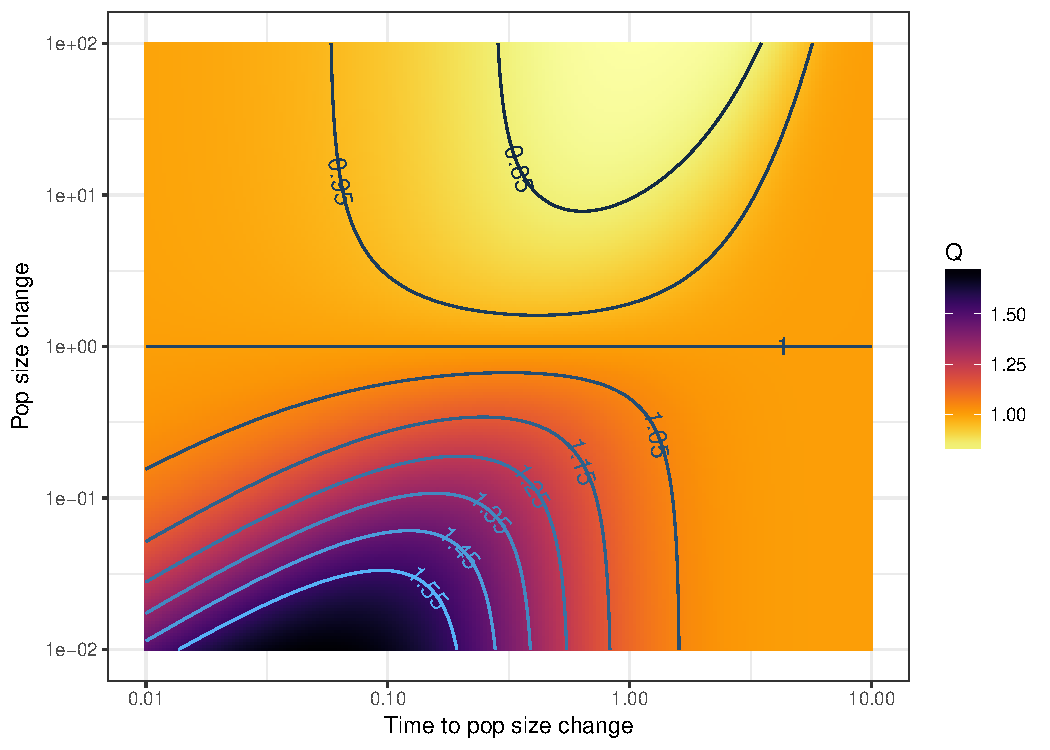
\includegraphics[width=0.9\textwidth]{Q_land.pdf}
  \caption{The scaling factor under different step population size
    changes.}
\end{figure}
Figure \ref{fig:Qland} shows how the expected excess in the fourth population
moment depends on the parameters $b$ and $c$ of the population size change. 
%%% mode: latex
%%% TeX-master: "notes.tex"
%%% End: 

\subsection{Differences in trait values}
\subsubsection{Kurtosis}
The distribution of a single trait value $Y$ is not very interesting because
this quantity cannot be observed. $Y$ gives the change in the trait value since
the most recent common ancestor of the sample, but since we don't know what that
value is we can't measure $Y$ in a sampled individual. What we can observe is
the differences in trait values between individuals, $Y_a-Y_b$. The results for
these differences are what one would expect given the distribution of the trait
values themselves. For instance, the second and fourth moments look exactly like
\eqref{eq:var} and \eqref{eq:mom4} if one substitutes twice the expected
coalescent time for the time to the most recent common ancestor of the sample.
One way to see this is by deriving the moment generating function for the
difference in trait values between two individuals. Using the same arguments 
that were used to derive \eqref{eq:sub} we get
\begin{align}
  \varphi_{Y_a-Y_b}(k) &= \int \int \prod_{\omega_1 \in \Omega_{a/b}}
                         e^{kY_{a,\omega_1}}P(Y_{a,\omega_1}=y_{a,\omega_1}|\mathbf{T}=\mathbf{t})dy_{a,\omega_1} \nonumber \\
  &\times \int \prod_{\omega_2 \in \Omega_{b/a}}
                         e^{-kY_{b,\omega_2}}P(Y_{b,\omega_2}=y_{b,\omega_2}|\mathbf{T}=\mathbf{t})dy_{a,\omega_2}
    P(\mathbf{T}=\mathbf{t})d\mathbf{t}.
\end{align}
From this we have removed all branches where $Y_a-Y_b$ is necessarily zero. This
includes branches that subtend both individuals and branches that subtend
neither individual. From this it is clear, as expected, that the distribution of
the trait difference between two individuals depends only on the distribution of
coalescence times for those individuals. Using the same result for compound
Poisson processes as before we get
\begin{align}
  \varphi_{Y_a-Y_b}(k) &= \int \prod_{\omega_1 \in \Omega_{a/b}} 
                         \exp\left( \T t_{\omega_1} \left( \Phi(k) - 1\right) \right) \nonumber \\
                       &\times \prod_{\omega_2 \in \Omega_{b/a}} 
                         \exp\left( \T t_{\omega_2} \left( \Phi(-k) - 1\right) \right) 
                         P(\mathbf{T}=\mathbf{t})d\mathbf{t}.
\end{align}
It is simple to use the low mutation rate approximation as in
\eqref{eq:mgf_approx_sub} to derive the second and fourth moments of the trait
difference. These are:
\begin{equation}
  E[(Y_a-Y_b)^2]=2L\T m_2 E[\tau_{a/b}].
\end{equation}
and
\begin{equation}
  E[(Y_a-Y_b)^4]=2L\T m_4 E[\tau_{a/b}] + 12L(L-1)(\T m_2 E[\tau_{a/b}])^2.
\end{equation}
The kurtosis is therefore
\begin{equation}
  \label{eq:diff_kurt}
  Kurt[Y_a-Y_b]=\frac{Kurt[M]}{2 L\T m_2 E[\tau_{a/b}]} + 3\left(1-\frac{1}{L} \right).
\end{equation}
Again, the kurtosis depends on the kurtosis of the mutational distribution and
the expected number of mutations affecting the trait. The kurtosis of the
difference between individuals in different populations will be smaller than for
individuals sampled within populations because the coalescence times will be
greater for individuals samples from different populations.
%%% Local Variables:
%%% TeX-master: "notes.tex"
%%% End:
\subsubsection{Cokurtosis}
Since the mean of a sample is uninformative, we have $n-1$ meaningful
observations in a sample of size $n$. Let $Y_0$ be the reference trait value and
$Y_1-Y_0,Y_2-Y_0,\ldots,y_{n-1}-Y_0$ are the observed trait differences. Let $X$
be the random vector of these differences. We are now interested in the
distribution of these differences. The moment generating function is
\begin{equation}
  \varphi_{\mathbf{X}}(\mathbf{k}) =
  \int e^{\mathbf{k} \cdot \mathbf{x} }
  \int P(\mathbf{X}=\mathbf{x}|\mathbf{T} = \mathbf{t})
  P(\mathbf{T}=\mathbf{t})d\mathbf{t}d\mathbf{x}.
\end{equation}
For the present we're going to look at $Cokurt[X_1,X_1,X_2,X_2]$, the cokurtosis between
two trait differences in a sample. This should hopefully tell us something about
the propensity of extreme trait values to be shared because of shared ancestry
of the individuals. The mgf for this is
\begin{equation}
  \int \int e^{k_1(y_a-y_0) + k_2(y_b-y_0)} P(Y_a-Y_0=y_a-y_0,Y_b-Y_0=y_b-y_0|\mathbf{T}-\mathbf{t})
  P(\mathbf{T}=\mathbf{t})d\mathbf{y}d\mathbf{t}.
\end{equation}
As before we can break this into different sections of the genealogy because the
changes in trait values along these branches are independent conditional on $T$.
Ignoring sets of branches where $Y_a-Y_0=Y_b-Y_0=0$, the relevant branch sets
are $(\Omega_{a/(b,0)},\Omega_{(0+b)/a},\Omega_{b/(0,a)},\Omega_{(0+a)/b},\Omega_{0/(a,b)},\Omega_{(a+b)/0})$.
Only considering these gives the following mgf
\begin{align*}
  \varphi_{Y_a-Y_0,Y_b-Y_0}(k_1,k_2) &=
  \int \prod_{\omega \in \Omega_{a/(0,b)}}\exp\left( \T t_{\omega} (\phi(k_1)-1) \right) \\
  &\times \prod_{\omega \in \Omega_{(0+b)/a}}\exp\left( \T t_{\omega} (\phi(-k_1)-1) \right) \\
  &\times \prod_{\omega \in \Omega_{b/(0,a)}}\exp\left( \T t_{\omega} (\phi(k_2)-1) \right) \\
  &\times \prod_{\omega \in \Omega_{(0+a)/b}}\exp\left( \T t_{\omega} (\phi(-k_2)-1) \right) \\
  &\times \prod_{\omega \in \Omega_{0/(a,b)}}\exp\left( \T t_{\omega} (\phi(-k_1-k_2)-1) \right) \\
  &\times \prod_{\omega \in \Omega_{(a+b)/0}}\exp\left( \T t_{\omega} (\phi(k_1+k_2)-1) \right)
  P(\mathbf{T}=\mathbf{t})d\mathbf{t}
\end{align*}
Application of the low mutation rate approximation and assuming that $m_1$ and
$m_3$ are zero gives
\begin{align*}
  (1 &+ \sum_{\omega \in \Omega_{a/(0,b)}} E[t_\omega] \T 
       \left[ \frac{m_2}{2} k_1^2 + \frac{m_4}{24}k_1^4\right] \\
     &+ \sum_{\omega \in \Omega_{(0+b)/a}} E[t_\omega] \T 
       \left[ \frac{m_2}{2} k_1^2 + \frac{m_4}{24}k_1^4 \right] \\
     &+ \sum_{\omega \in \Omega_{b/(0,a)}} E[t_\omega] \T
       \left[ \frac{m_2}{2} k_2^2 + \frac{m_4}{24}k_2^4 \right] \\
     &+ \sum_{\omega \in \Omega_{(0+a)/b}} E[t_\omega] \T 
       \left[ \frac{m_2}{2} k_2^2 + \frac{m_4}{24}k_2^4 \right] \\
     &+ \sum_{\omega \in \Omega_{0/(a,b)}} E[t_\omega] \T
       \left[ \frac{m_2}{2} (k_1 + k_2)^2 + \frac{m_4}{24}(k_1 + k_2)^4\right] \\
     &+ \sum_{\omega \in \Omega_{(a+b)/0}} E[t_\omega] \T 
       \left[ \frac{m_2}{2} (k_1 + k_2)^2 + \frac{m_4}{24}(k_1 + k_2)^4 \right])^L.
\end{align*}
If we ignore terms that won't contribute to the cokurtosis and do some grouping
we get
\begin{align*}
  (1 &+ \sum_{\omega \in \Omega_{0/a}} E[t_\omega] \T \frac{m_2}{2}k_1^2 \\
     &+ \sum_{\omega \in \Omega_{a/0}} E[t_\omega] \T \frac{m_2}{2}k_1^2 \\
     &+ \sum_{\omega \in \Omega_{0/b}} E[t_\omega] \T \frac{m_2}{2}k_2^2 \\
     &+ \sum_{\omega \in \Omega_{b/0}} E[t_\omega] \T \frac{m_2}{2}k_2^2 \\
     &+ \sum_{\omega \in \Omega_{0/(a,b)}} E[t_\omega] \T 
       \left[ \frac{m_2}{2} 2k_1k_2 + \frac{m_4}{24}k_1^2k_2^2\right]\\
     &+ \sum_{\omega \in \Omega_{(a,b)/0}} E[t_\omega] \T 
       \left[ \frac{m_2}{2} 2k_1k_2 + \frac{m_4}{24}k_1^2k_2^2\right])^L.
\end{align*}
These sums over internal branches can be interpreted in terms of coalescence
times. 
\begin{align*}
(1 &+ 2E[\tau_{a/0}] \T \frac{m_2}{2}k_1^2 \\
   &+ 2E[\tau_{b/0}] \T \frac{m_2}{2}k_2^2 \\
   &+ E[\tau_{0/(a,b)}] \T \left[ \frac{m_2}{2} 2k_1k_2 + \frac{m_4}{24}6k_1^2k_2^2\right]\\
   &+ E[\tau_{(a,b)/0}] \T \left[ \frac{m_2}{2} 2k_1k_2 + \frac{m_4}{24}6k_1^2k_2^2\right])^L.
\end{align*}y
As before $E[\tau_{a/0}]$ is the expected coalescence time between individuals
$a$ and $0$. $E[\tau_{0/(a,b)}]$ is the expected total branch length subtending
individual $0$ before this lineage coalesces with either $a$ or $b$.
$E[\tau_{(a,b)/0}]$ is the expected total branch length subtending both $a$ and
$b$ before either coalesces with $0$. This is a much less common a genealogical
quantity than the expected coalescent time, but it seems to make sense in this
context. Taking the appropriate derivatives we get
\begin{align}
\label{eq:diffcokurt}
  E[Y_a-Y_0,Y_b-Y_0] &= 4L(L-1)E[\tau_{a/0}]E[\tau_{b/0}]\left(\T\right)^2m_2^2 \nonumber \\
                     &+ 2L(L-1)(E[\tau_{0/(a,b)}]+E[\tau_{(a,b)/0}])^2\left( \T \right)^2 m_2^2 \nonumber \\
                     &+ L E[\tau_{0/(a,b)}] \T m_4 + L E[\tau_{(a,b)/0}] \T m_4.
\end{align}
The cokurtosis is then 
\begin{equation}
  \left( 1 - \frac{1}{L} \right) \left( 1 + 
  \frac{(E[\tau_{0/(a,b)}]+E[\tau_{(a,b)/0}])^2}{2E[\tau_{a/0}]E[\tau_{b/0}]} \right)+ 
  \frac{Kurt[M]\left(E[\tau_{0/(a,b)}] +  E[\tau_{(a,b)/0}]\right)}{4L \T E[\tau_{a/0}]E[\tau_{b/0}]}.
\end{equation}
The cokurtosis of a multivariate normal distribution is $1+2\rho$ where $\rho$
is the correlation between the two variables. With this in mind we can
rewrite \eqref{eq:diffcokurt} as
\begin{equation}
  \left( 1 - \frac{1}{L} \right) \left( 1 + 
  2\frac{(E[\tau_{0/(a,b)}]+E[\tau_{(a,b)/0}])^2}{4E[\tau_{a/0}]E[\tau_{b/0}]} \right)+ 
  \frac{Kurt[M]\left(E[\tau_{0/(a,b)}] +  E[\tau_{(a,b)/0}]\right)}{4L \T E[\tau_{a/0}]E[\tau_{b/0}]}.
\end{equation}
Here,
$\frac{(E[\tau_{0/(a,b)}]+E[\tau_{(a,b)/0}])^2}{4E[\tau_{a/0}]E[\tau_{b/0}]}$
makes sense as the correlation between $Y_a-Y_0$ and
$Y_b-Y_0$. \eqref{eq:diffcokurt} therefore has the same form as the other
kurtosis formulas where the excess kurtosis above the normal expectation is
proportional to the mutational kurtosis.
%%% Local Variables:
%%% TeX-master: "notes.tex"
%%% End:

\subsection{Genealogy moment generating functions for structured populations}
\citet{Lohse2011} found general forms for the generating functions of
genealogies. In a coalescent model where events $i$ occur at rate $ \lambda_i $,
the moment generating function for the genealogy can be written as
\begin{equation}
  \varphi_{T}\left[ \mathbf{T} \right] = \frac{
    \sum_i \lambda_i \varphi_i[\mathbf{s}]}{
    \sum_i \lambda_i + \sum_{|\omega|=1}s_{\omega}}.
\end{equation}
This is a convolution of the time to the first event with a mixture of times
after the first event, where the mixture is over all possible next events. We
can apply this equation to a generalized structured population model where, $M$
is the number of demes, $m_{i,j}$ is the migration rate from deme $i$ to deme
$j$, $\eta_i$ is the coalescent rate within deme $i$, and
$\Omega = \{ \Omega_1, \Omega_2, \ldots , \Omega_M \}$ is the collection of
lineages currently active in each deme. In this model, events occur at rate
\begin{equation}
  \sum_{i=1}^M \binom{|\Omega_i|}{2}\eta_i + \sum_{(i,j:i \neq j)} m_{i,j}|\Omega_i|,
\end{equation}
where the first term is due to coalescence events and the second term is due to
migration events. We first define operations on $\Omega$ due to these events. A
event of lineage $\omega$ migrating from deme $i$ to deme $j$ would be
represented as
\begin{equation*}
  \Omega\left( i  :-\omega,j: + \omega \right) := \{ \Omega\backslash \{\Omega_i, \Omega_j \} \} \cup
  \{\Omega_j\backslash \omega, \Omega_i \cup \omega \}. 
\end{equation*}
A coalescent event of lineages $x$ and $y$ in deme $i$ would be
written as 
\begin{equation*}
  \Omega(i:a \cup b):=\{ \Omega \backslash \Omega)_i \}\cup\{ \{\Omega_i \cup ab \}\backslash \{ a,b \}\}
\end{equation*}
The overall generating function is then
\begin{align}
  \varphi_{\mathbf{T}}^{\Omega}(\mathbf{s}) &=
                                              \left( \sum_{i=1}^M \binom{|\Omega_i|}{2}\eta_i  + \sum_{(i,j:i \neq j)} m_{i,j}|\Omega_i| -
                                              \sum_{i=1}^M \sum_{\omega \in \Omega_i}s_{\omega}\right)^{-1} \\
                                            &\times \left( \sum_{i=1}^M \eta_i \sum_{(a,b) \in \Omega_i:a \neq b}
                                              \varphi_{\mathbf{T}}^{\Omega(i:a \cup b)}(\mathbf{s}) + 
                                              \sum_{(i,j):i\neq j}m_{i,j}\sum_{\omega \in \Omega_i} \varphi_{\mathbf{T}}^{\Omega\left( i :-\omega, j: + \omega \right)}(\mathbf{s})\right).
\end{align}b
If there are $N$ sample lineages, this gives a system of $M^{\binom{N}{2}-1}$
equations which is a fuckton.

%%% Local Variables:
%%% TeX-master: "notes.tex"
%%% End:

\subsection{Trait value moment generating functions for structured populations}
To convert this into a moment generating function for branch lengths we would make the substitution specified by
equation \ref{eq:sub}. This gives 
\begin{align}
  \label{eq:gensub}
  \varphi_{\mathbf{T}}^{\Omega}(\mathbf{k}) &=
  \left( \sum_{i=1}^M \binom{|\Omega_i|}{2}\eta_i  + \sum_{(i,j:i \neq j)} m_{i,j}|\Omega_i| -
  \sum_{i=1}^M \sum_{\omega \in \Omega_i} \T\left( \psi\left(\sum_{a \in \omega}k_{a}\right) -1\right)\right)^{-1} \\
  &\times \left( \sum_{i=1}^M \eta_i \sum_{(a,b) \in \Omega_i:a \neq b}
  \varphi_{\mathbf{T}}^{\Omega(i:a \cup b)}(\mathbf{k}) + 
  \sum_{(i,j):i\neq j}m_{i,j}\sum_{\omega \in \Omega_i} \varphi_{\mathbf{T}}^{\Omega\left( i :-\omega, j: + \omega \right)}(\mathbf{k})\right).
\end{align}
If we are only interested in calculating particular moments of this distribution we can simplify this expression
substantially. For instance, if we want the second moment of $k$, then this depends only on the expected TMRCA. We will
be taking the second derivative of $\varphi$ with respect to an arbitrary $k_i$ and also substituting zero for each
$k_i$. For solving the recursion which we will then take the second derivative of and evaluate at zero, we define a 
function $g(\mathbf{n}, k)$. The recursion for this function is 
\begin{align}
  \label{eq:grecur}
  g(\mathbf{n}, k) &= \left( \sum_{i=1}^M \binom{n_i}{2}\eta(i) + \sum_{i=1}^Mn_i\sum_{j=1}^Mm(i,j) + 
    \T \frac{k^2}{2}m_2 \right)^{-1} \nonumber \\
  &\times \left( \sum_{i=1}^M \binom{n_i}{2} \eta(i) g(c(i,\mathbf{n}), k) + 
  \sum_{i=1}^Mn_i\sum_{j=1}^Mm(i,j)g(e(i,j,\mathbf{n}),k)\right).
\end{align}
In this, $c(i,\mathbf{n})$ is a coalescent operation that removes a lineage from deme $i$. and $e(i,j,\mathbf{n})$ is a
migration operation that moves a lineage from deme $i$ to deme $j$. 

%%% Local Variables: 
%%% mode: latex
%%% TeX-master: "notes.tex"
%%% End: 

\subsection{An example of the infinitesimal limit in panmictic populations}
We look at an example from a panmictic population to see how the genealogy generates a correlation structure among the
samples. In particular, we take limits corresponding to an infinitesimal model and show that this results in multivariate 
normal distribution. 

%%% Local Variables: 
%%% mode: latex
%%% TeX-master: "notes.tex"
%%% End: 

\subsection{The distribution of individual differences}
In any sample, the absolute phenotypic values will not be meaningful. It is differences between individuals sampled from
various sub populations that are of interest to us. We are therefore interested in the joint distribution of $Y_i-Y-j$
for each pair of individuals in the sample. Using the infinitesimal model with a distribution of mutational effects
centered at zero the differences should have a multivariate normal distribution with mean zero. What matters is the
covariances of the differences.
\begin{equation}
  \label{eq:cov}
  Cov[Y_1-Y_2,Y_3-Y_4]=Cov[Y_1,Y_3]+Cov[Y_2,Y_4]-Cov[Y_1,Y_4]-Cov[Y_2,Y_3]
\end{equation}
We know from previous results that $Cov[Y_1,Y_2]$ is proportional to the shared branch length of individuals $1$ and $2$
before the most recent common ancestor of the sample. We therefore have
\begin{equation}
  \label{eq:covprop}
  Cov[Y_1,Y_2] \propto E[T_{MRCA}]-E[\tau_{1,2}],
\end{equation}
and
\begin{equation}
  \label{eq:covcoal}
  Cov[Y_1-Y_2,Y_3-Y_4] \propto E[\tau_{1,4}] + E[\tau_{2,3}] - E[\tau_{1,3}] - E[\tau_{2,4}].
\end{equation}
Where $\tau_{1,2}$ is the expected coalescence time of individuals $1$ and $2$. 
%%% Local Variables: 
%%% mode: latex
%%% TeX-master: "notes.tex"
%%% End: 

\subsubsection{The sampling distribution of $Q_{ST}$ under the infinitesimal model}
The $Q_{ST}$ statistic measures how much of the phenotypic variation in a
structure population is partitioned between groups. $Q_{ST}$ is defined as 
\begin{equation}
  \label{eq:qst}
  Q_{ST} := \frac{V_{\text{between}}}{V_{\text{between}} + V_{\text{within}}}.
\end{equation}
In the usual analysis of variance framework, the variance between $K$
populations is $\frac{1}{K} \sum \left( \bar{Y}_i - \bar{Y}\right)^2$ and the
variance within groups is $\frac{1}{\sum N_k} \sum_i \sum_j \left( Y_{i,j} - \bar{Y}_i\right)^2$.
To examine the distribution of $Q_{ST}$ at the population level one can
figure out what the distributions of $V_{between}$ and $V_{within}$ are over
evolutionary realizations. Even if the full distribution of $Q_{ST}$ does not have
and analytic form, we can sample from the distributions of the variance to calculate
tail probabilities.

Under the infinitesimal model, each $Y_{i,j}$ is normally distributed, so the
means are therefore also normal. When the population size is large enough,
$(Y_{i,j} - \bar{Y}_i)^2$ and $(Y_{j,l} - \bar{Y}_j)^2$ are nearly uncorrelated
both within and between populations because each individual contributes little
to the population means. $V_{within}$ is therefore a sum of squared independent
normal random variables with mean zero. With enough individuals in the whole
population, the central limit theorem kicks in and the variance is order $1/\sum N_k$.
The mean value of $\E[(Y_{i,j} - \bar{Y}_i)^2]$ is $\sigma^2E[\tau_{i,i}]$. 
We can thus treat $V_{within}$ as a constant with value $\frac{\sum N_k \E[\tau_{k,k}]}{\sum N_k}$. 
If $c_k$ is the fraction of the total population in group $k$, then $V_{within}=\sum c_k \E[\tau_{k,k}]$. 
This brings up the issue that the fraction that each group makes up of the total
population is unlikely to be known. This makes thinking about $Q_{ST}$ as a population
parameter a bit tricky. I think it is best to think of it as an idealized sample value
when a large and equal number of samples is taken from each population.

In the variance between groups, the $(\bar{Y}_i - \bar{Y})^2$ terms are
correlated. The sum of these will have a generalized chi-square distribution. We
could sample from this distribution by simulating the $\bar{Y}_i - \bar{Y}$ from
a multivariate normal distribution and adding the squared values. The covariance
matrix for this distribution is
\begin{equation}
  \Cov[\bar{Y}_i - \bar{Y}, \bar{Y}_j - \bar{Y}] = \sigma^2\left(
  \E[\tau_{i,\cdot}] + \E[\tau_{j,\cdot}] - \E[\tau_{\cdot,\cdot}] -
  \E[\tau_{i,j}]\right). 
\end{equation}

%%% Local Variables: 
%%% mode: latex
%%% TeX-master: "notes.tex"
%%% End: 

\section{Dominance}
\subsection{The individual variance}
When modeling dominance each individual receives two copies of alleles from the
population. These may contain the same or different alleles. An individual's
genotype is then made up of contributions from $L$ loci.
\begin{equation}
  Y=\sum_{l=1}^L f(Y_{l,1},Y_{l,2}).
\end{equation}
The function $f$ is a function that describes the ``dominance'' relationship for
the trait. It is natural to set $f(0,0)=0$ so that there is no effect when an
individual receives no mutations at a locus. If we assume that each locus has an
independent genealogy, then the variance of $Y$ can be computed by calculating
$\Var[f(Y_{l,1}.Y_{l,2})]$. One way to do this is by using the law of total
variance and conditioning on the mutational configuration at the locus.
\begin{equation*}
  \E[ \Var(f(Y_{l,1},Y_{l,2}) | \mbox{mutation} )] +
  \Var( \E[ f(Y_{l,1}.Y_{l,2}) | \mbox{mutation} ]).
\end{equation*}
The second term here will be zero if the mutational distribution and
transformation $f$ are both symmetric. We'll then assume that at most one
mutation occurs per locus genealogy. This means it is only necessary to
calculate $\Var(f(Y_{l,1}.Y_{l,2})| 1 \mbox{ mutation}))$ and
$\Var(f(Y_{l,1}.Y_{l,2})| 2 \mbox{ mutations}))$.

To proceed one will need to assume a specific form for $f$. A very simple
function is
\begin{equation}
  f(Y_{l,1}.Y_{l,2}) =
  \begin{cases}
    bY_{l,1}, & \text{if } Y_{l,2} = 1\\
    2Y_{l,1}, & \text{if } Y_{l,2} \neq 1.
  \end{cases}
\end{equation}
In this model every mutation has the same degree of dominance regardless of how
big of an effect it has on the trait. More complicated models are possible, but
this one is good so far for building intuition. Under this model,
\begin{equation*}
  \Var(f(Y_{l,1}.Y_{l,2})| 1 \mbox{ mutation})) = b^2m_2,
\end{equation*}
and
\begin{equation*}
  \Var(f(Y_{l,1}.Y_{l,2})| 2 \mbox{ mutations})) = 4m_2.
\end{equation*}

The expected variance at a locus is then
\begin{equation*}
  \Var(f(Y_{l,1}.Y_{l,2})| 1 \mbox{ mutation}))\P(1 \mbox{ mutation}) +
  \Var(f(Y_{l,1}.Y_{l,2})| 2 \mbox{ mutations}))\P(2 \mbox{ mutations}).
\end{equation*}
Which evaluates overall to
\begin{equation}
  2\T \tau_{2,2} b^2 m_2 + \T(T_{MRCA} - \tau_{2,2})4m_2.
\end{equation}
We only need to take the expectation over genealogies at each locus to finish
the derivation
%%% Local Variables:
%%% TeX-master: "notes.tex"
%%% End:

\subsection{The population variance}
The variance in trait values between individuals determines the expected
variance in the population. This variance can be written as
\begin{equation*}
  \Var( \sum_{l=1}^L f(Y_{1,l,1},Y_{1,l,2}) - \sum_{l=1}^L f(Y_{2,l,1},Y_{2,l,2}) ).
\end{equation*}
The important term to calculate is
$\Cov(f(Y_{1,l,1},Y_{1,l,2}),f(Y_{2,l,1},Y_{2,l,2})) = \E[f(Y_{1,l,1},Y_{1,l,2}),f(Y_{2,l,1},Y_{2,l,2})]$.
We can use the law of total expectation to calculate this again
conditioning on different mutational configurations. The configurations
that lead to a nonzero expectation if one mutation occurs is present in each individual,
three mutations occur, or four mutations occur. There are four ways for the two individuals
to each have one mutant copy. When this occurs the expected product will be $b^2m_w$. There
are four ways for a mutation to be present in three copies and when this occurs the expected
product will be $2b m_2$. There is one way to have a mutation present in all four copies
and the expected product is $4m_2$.

We can then us the probability of each type of mutational configuration occurring
to calculate the covariance. 

%%% Local Variables:
%%% TeX-master: "notes.tex"
%%% End:

\section{Epistasis}
\subsection{Nonlinear transformation of trait values}
\textit{For now this section is exploratory, so the notation will likely differ
  from the rest of the notes.}

One simple form of epistasis is a nonlinear transformation of the individual
trait values. If $X_i$ are the genetic values contributed by each of $L$ loci,
then the trait value of an individual would be
\begin{equation*}
  Y = f\left(\sum_{i=1}^{L} X_i\right).
\end{equation*}
Under the infinitesimal model the $\sum X_i$ are normally distributed. As a
nonlinear transformation of a normal variable, $Y$ will not be normally
distributed. However, we can still investigate its first two moments to see the
effects of epistasis. If $f$ is very complicated then this could be a very
difficult thing to do. We can start by taking a second-order Taylor expansion of
$f$. Expanding $f$ around zero gives
\begin{equation*}
  Y \approx f(0) + f'(0)\sum_{i=1}^L X_i + \frac{1}{2}f''(0)\left(\sum_{i=1}^L X_i\right)^2.
\end{equation*}
This assumes that the curvature is the same in each direction, which is not a
crazy assumption. Let $f(0)=0$, $f'(0)=1$, and $f''(0)=\epsilon$. When deriving
stuff under the assumption that $\sum X_i$ is normal, let $X=\sum X_i$.

The first thing to investigate is the effect of weak epistasis on the variance.
This is
\begin{equation*}
  \Var[X + \epsilon X^2] = \Var[X] + \epsilon \Var[X^2] + 2 \epsilon \Cov[X,X^2].  
\end{equation*}
Using standard results on the normal distribution and previously derived
results, $\Var[X]=\mu \E T_{MRCA}$, $\Var[X^2]=2\sigma^4\E T_{MRCA}^2+4\sigma^2\mu^2 \E T_{MRCA}^3$,
and $\Cov[X,X^2]=2\mu\sigma^2 \E T_{MRCA}$. Putting this together and setting $\mu=0$ gives the
variance
\begin{equation}
  \Var[X + \epsilon X^2] = \sigma^2\E T_{MRCA} + 2\epsilon \sigma^2 \E [T_{MRCA}]^2.
\end{equation}
The corresponding expectation is
\begin{equation}
  \E[X + \epsilon X^2] = \mu \E T_{MRCA} + \epsilon \sigma^2 \E T_{MRCA}.
\end{equation}

The covariance can be derived in a similar manner.
\begin{equation}
  \Cov[X_1 + \epsilon X_1^2,X_2 + \epsilon X_2^2] = \Cov[X_1,X_2] + \epsilon
  \Cov[X_1,X_2^2] + \epsilon \Cov[X_1^2,X_2] + \epsilon^2 \Cov[X_1^2,X_2^2].
\end{equation}
If $\mu=0$ the second and third term are zero and the fourth term is
\begin{equation*}
  2\sigma^4\left( \E T_{MRCA} - \tau_{1,2} \right)^2.
\end{equation*}
This ultimately gives
\begin{equation}
  \Cov[X_1 + \epsilon X_1^2,X_2 + \epsilon X_2^2] = \sigma^2\left(\E T_{MRCA} -
  \tau_{1,2}\right) + 2\epsilon^2 \sigma^4\left(\E T_{MRCA} -
  \tau_{1,2}\right)^2.
\end{equation}

Additionally, the variance in the difference in trait values between sampled
individuals is a good measure of the amount of variation in the population.
Indeed, as long as the individuals are exchangeable this is proportional to the
expected variance in a large population.
\begin{equation*}
  \Var[X_1 - \epsilon X_1^2 - X_2 - \epsilon X_2^2] =
  \Var[X_1 + \epsilon X_1^2] + \Var[X_2 + \epsilon X_2^2] -
  2\Cov[X_1 + \epsilon X_1^2, X_2 + \epsilon X_2^2].
\end{equation*}
Again, if $\mu=0$ we can use previous results to get
\begin{equation*}
  \Var[X_1 - \epsilon X_1^2 - X_2 - \epsilon X_2^2] =
  2\sigma^2\tau_{1,2} + 4\sigma^4\epsilon \left( \E[T_{MRCA}]^2 -
  \epsilon \sigma^2 (\E T_{MRCA} - \tau_{1,2})^2 \right).
\end{equation*}
What is interesting about this is that we can see when the expected population
variance will be greater than that without epistasis. This is the case when
\begin{equation}
  \frac{\E[T_{MRCA}]^2}{\E[T_{MRCA}-\tau_{1,2}]^2} > \epsilon \sigma^2
\end{equation}
When $\epsilon < 0$ the variance is always less than under the additive case. 
%%% Local Variables:
%%% TeX-master: "notes.tex"
%%% End:


\section{Selection}
\subsection{Selection on a polygenic character}
We have investigated the fact that, when the number of loci expected to
experience mutations affecting a trait is low, the kurtosis is higher than that
for a normal distribution. This kurtosis is over evolutionary realizations. If
we were to replay evolution then individuals would have more extreme values
relative to the variance of the distribution than under a normal distribution.
It is worth asking how this affects selection. Even though the models so far
have been strictly neutral, we can imagine selection acting on the population
and producing a change in the mean an variance of trait values. The classical
theory of quantitative genetics assumes a normal distribution of breeding values
in the population. In one of a series of papers, \citet{Turelli1990} extended
the theory of selection on a polygenic character to a more realistic model of
multilocus population genetics. One conclusion of this work is that selection
can cause deviations from normality in higher order moments of the distribution
of breeding values, affecting the progress of selection.

A central result of \citet{Turelli1990} is that the change in the mean phenotype
due to one generation of selection is

\begin{equation}
  \Delta \bar{Z} = V_gL_1 + M_{3,g}L_2 + \gamma_4V^2_gL_3 +
  \left( M_{5,g}-4M_{3,g}V_g\right)L_4 + \ldots.
\end{equation}

Here, $Z$ refers to a phenotypic value which has an environmental component as
opposed the breeding value $Y$ which is due entirely to genetics. $V_g$ is the
variance in breeding values in the population and $\gamma_4$ is the excess
kurtosis above a normal distribution. The terms $M_{i,g}$ are the $i^{th}$
central moments of the breeding value distribution in the population. The terms
$L_i$ describe the effect of selection on the breeding values. These are the
selection gradients in terms of the genotypic moments.

\begin{equation}
  L_i = \frac{\partial \ln(\bar{w})}{\partial M_{i,g}}
\end{equation}

and

\begin{equation}
  L_1 = \frac{\partial \ln(\bar{w})}{\partial \bar{Y}}.
\end{equation}

What we can tell immediately from these equations is that the importance of
higher order moments of the breeding value distribution depends on the specific
fitness function. For instances, the effect of the skew of the breeding value
distribution $M_{3,g}$ depends on the effect on the mean fitness of changing the
variance of the breeding values $\frac{\partial \ln(\bar{w})}{V_g}$. Each of the
$L_i$ terms correspond to the effects on mean fitness of changing one moment
while holding the others constant. Therefore, whether or not the excess kurtosis
that arises due to a sparse trait architecture has a meaningful effect on the
response to selection depends on the precise shape of that selection.
\citet{Turelli1990} use trick to calculate the $L_i$. By taking a Taylor series
expansion of $w_g(Y)$ they get

\begin{equation}
  \label{eq:wbar}
  \bar{w} = w_g(\bar{Z}) + \sum_{i=2}^\infty \frac{M_{i,g}w^{(i)}_g(\bar{Z})}{i!}.
\end{equation}

Differentiating this gives

\begin{equation}
  \label{eq:l1}
  L_1= \frac{w_g^{(1)}(\bar{Z)}}{\bar{w}} + \sum_{i=2}^\infty \frac{ M_{i,g}w^{(i+1)}( \bar{Z} ) }{ i! \bar{w} },
\end{equation}

and

\begin{equation}
  \label{eq:li}
  L_i = \frac{w_g^{(i)}(\bar{Z})}{i!\bar{w}}.
\end{equation}

What this shows is that it is sufficient when calculating $L_i$ to calculate the
$i^{th}$ derivative of $w_g$ and evaluate this at the population mean.

%%% Local Variables:
%%% TeX-master: "notes.tex"
%%% End:

\subsection{Exponential selection}
One simple fitness function is exponential directional selection:

\begin{equation}
  w(z) = e^{sz}.
\end{equation}

This fitness function has a number of nice properties. Fitness is multiplicative
across loci so it does not lead to a build up of linkage disequilibrium.
Additionally, the ratio of fitnesses between two phenotypes does not depend on
the reference from which one measures them. \citet{Turelli1990} investigate
exponential directional selection. They calculate

\begin{equation}
  \bar{w} = e^{sz} \exp \left( \frac{s^2V_e}{2} \right)
  \left( 1 + \sum_{i=2}^{\infty} \frac{s^iM_{i,g}}{i!} \right),
\end{equation}

\begin{equation}
  L_1 = s, \qquad L_2\approx s^2, \qquad \text{and} \qquad L_k \approx 0 \qquad \text{for} \qquad k \geq 3.
\end{equation}

The approximations ignore terms of order $s^2$. Thanks to \eqref{eq:dz} we can
see that only the variance and skew of the breeding values will affect the response to selection in this case. 

%%% Local Variables:
%%% TeX-master: "notes.tex"
%%% End:

\subsection{Cubic selection}
The population kurtosis may become more important if we want to consider
selection where the fitness function is cubic on the breeding values. Such a
fitness function would have the form
\begin{equation}
  \label{eq:cubsel}
  W_g(Y) = b_0 + b_3(Y-\bar{Y})^3.
\end{equation}
This fitness function now models selection on differences from the current mean
breeding value in the population. This is not the most realistic scenario
because this mean will have diverged since the most recent common ancestor of
the population in the absence of stabilizing selection. The reference point
which selection sees as the center is therefore somewhat arbitrary. There's no
good reason for this to be the population mean, but it's also not totally
unreasonable. Another thing we need to consider about the cubic selection
function is that it can give negative values for fitness, which is something we
clearly don't want. We therefore must assume that the degree of cubic selection,
$b_3$ is not too large relative to fitness value at the population mean, $b_0$.
Figure \ref{fig:cubshape} shows a few examples of cubic fitness functions
applied to a simulated population with mean breeding value around four.
Selection gets very steep as $b_3$ increases and one ends up with negative
fitness values that are then set to zero

\begin{figure}
  \centering
  \includegraphics[width=0.6\textwidth]{cub_shape.pdf}
  \caption{Cubic fitness functions with $b_0=50$ applied to a random population
    with 2000 individuals, 100 loci, and a standard deviation of mutational
    effects of one.}
  \label{fig:cubshape}
\end{figure}

Note that we're now considering selection directly on breeding values rather
than starting with selection on phenotypic values and deriving selection on
breeding values assuming a Gaussian distribution for environmental effects. We
might justify this by saying that this should capture the effect of that portion
of the overall fitness function which has a cubic shape with respect to the
breeding values.

Applying \eqref{eq:Li}, \eqref{eq:wbar}, and \eqref{eq:wbar} to
\eqref{eq:cubsel} we get
\begin{equation}
  \bar{w} = b_0 + M_{3,g}b_3,
\end{equation}
\begin{equation}
  L_1 = \frac{3V_gb_3}{\bar{w}},
\end{equation}
\begin{equation}
  L_2 = 0,
\end{equation}
\begin{equation}
  L_3 = \frac{b_3}{\bar{w}}.
\end{equation}
After combining these all into \eqref{eq:dz} we get
\begin{equation}
  \label{eq:cubresp}
  \Delta \bar{Z} = \frac{3 V_g^2b_3 + (M_{4,g}-3V_g^2)b_3}{b_0 + M_{3,g}b_3} =
  \frac{M_{4,g}b_3/b_0}{1 + M_{3,g}b_3/b_0} = \frac{M_{4,g}\beta}{1 +
    M_{3,g}\beta}.
\end{equation}
We can see that the response to cubic selection depends only on $\beta$, the
ratio of the steepness of cubic selction to the baseline fitness, as well as the
third and fourth moments of the distribution of breeding values. In general the
response to cubic selection is linear with respect to the fourth moment of the
distribution of breeding values and hence the kurtosis.

Since the theory of \citet{Turelli1990} is for weak selection, we must
investigate the range of selection strengths for which \eqref{eq:cubsel}
predicts the average response to selection. To do this, for a range of $\beta$
values I simulated 50 populations with 2000 haploid individuals each and a
mutational standard deviation of one. I drew individuals for the next generation
according to fitness values from \eqref{eq:cubsel} and compared the change in
phenotype to that predicted by \eqref{eq:cubresp}. The results of this
experiment are shown in Figure \ref{fig:incrcub}. The weak selection
approximations of \citet{Turelli1990} begin to break down for $\beta$ greater
than $0.001$, which as Figure \ref{fig:cubshape} shows, corresponds to quite
strong selection. 

\begin{figure}
  \centering
  \label{fig:incrcub}
  \includegraphics[width=\textwidth]{cubic_sel.pdf}
    \caption{Simulation results comparing the response to varying strengths of
    cubic selection to the expected response under weak selection theory given
    by \eqref{eq:cubresp}. Simulation realizations for a given $\beta$ have
    different responses to selection because of differences in the fourth moment
    of breeding values arising by chance. Lines show the one-to-one relationship
    for comparison.}
\end{figure}
%%% Local Variables:
%%% TeX-master: "notes.tex"
%%% End:


\clearpage
\bibliographystyle{genetics}
\bibliography{quant_gen}

\section{Supplement}
\subsection{Additional steps for some derivations}
In the derivation of \eqref{eq:m31}, how the second term is arrived at is not
immediately obvious. To see where this comes from, consider the two types of
terms within \eqref{eq_mgf_approx_sum} that will contribute $k_a^3k_b$ from
pairs of branches. These are those pairs where both contain $a$ and $b$, and
those pairs where one contains $a$ and $b$ and the other contains $a$ only.
Pairs with the same branch repeated twice have multiplicity $L(L-1)/2$ and pairs
with two different branches have multiplicity $L(L-1)$. Branch pairs where both
contain $a$ and $b$ have $4k_a^3k_b$ because this term can be made four times
from $(k_a+k_b)^4$, and branch pairs where one contains $a$ and the other $a$
and $b$ have $2k_a^3k_b$ because this term can be made two ways from
$k_a^2(k_a+k_b)^2$. These two sets of pairs are
\begin{equation*}
  \frac{L(L-1)}{2} \left( \T \frac{m_2}{2}\right)^2 2k_a^2\times 2k_ak_b
  \left( \sum_{\omega: a,b \in \omega} E[t_\omega] \right)^2
\end{equation*}
and
\begin{equation*}
  L(L-1) \left( \T \frac{m_2}{2}\right)^2 k_a^2\times 2k_ak_b
  \left( \sum_{\omega: a,b \in \omega} E[t_\omega] \right)\left( \sum_{\omega: a/b \in \omega} E[t_\omega] \right).
\end{equation*}
These two can clearly be added together to yield
\begin{equation*}
  L(L-1) \left( \T \frac{m_2}{2}\right)^2 k_a^2\times 2k_ak_b
  \left( \sum_{\omega: a,b \in \omega} E[t_\omega] \right)\left( \sum_{\omega: a \in \omega} E[t_\omega] \right).
\end{equation*}

The derivation of \eqref{eq:m211} is even more challenging because more
potential branch pairs need to be considered between the three descendants
included in the moment. As before pairs containing the same branch twice have a
multiplicity of $L(L-1)/2$ while pairs containing two different branches have a
multiplicity of $L(L-1)$. Depending on what individuals are on each branch
$k_a^2k_bk_c$ will also have a different coefficient. I'll consider each
possible type of pair in sequence then add them together at the end.

\begin{flushleft}
  \textbf{$a$, $b$, and $c$ are present on all branches}\\
\end{flushleft}
Since all individuals are present on both branches, the coefficient of
$k_a^2k_bk_c$ is multinomial ($12$). The term for this set of pairs is then
\begin{equation*}
  \frac{L(L-1)}{2} 12 k_a^2k_bk_c \left( \sum_{\omega: a,b,c \in \omega} E[t_\omega] \right)^2.
\end{equation*}
\begin{flushleft}
  \textbf{Only $a$ and $b$ are on one branch while $a$, $b$ and $c$ are on the other}\\
\end{flushleft}
In this case $k_a^2k_bk_c$ has coefficient $6$. Since these are non-overlapping
sets of branches we get
\begin{equation*}
  L(L-1) 6 k_a^2k_bk_c \left( \sum_{\omega: a,b/c \in \omega} E[t_\omega] \right)
  \left( \sum_{\omega: a,b,c \in \omega} E[t_\omega] \right).
\end{equation*}
\begin{flushleft}
  \textbf{Only $a$ and $c$ are on one branch while $a$, $b$ and $c$ are on the other}\\
\end{flushleft}
This is the same as above.
\begin{equation*}
  L(L-1) 6 k_a^2k_bk_c \left( \sum_{\omega: a,c/b \in \omega} E[t_\omega] \right)
  \left( \sum_{\omega: a,b,c \in \omega} E[t_\omega] \right).
\end{equation*}
\begin{flushleft}
  \textbf{Only $a$ is present on one branch while $a$, $b$ and $c$ are on the other}\\
\end{flushleft}
In this case $k_a^2k_bk_c$ has coefficient $2$. These branches contain
non-overlapping sets of descendants again so we can write
\begin{equation*}
  L(L-1) 2 k_a^2k_bk_c \left( \sum_{\omega: a/b,c \in \omega} E[t_\omega] \right)
  \left( \sum_{\omega: a,b,c \in \omega} E[t_\omega] \right).
\end{equation*}
\begin{flushleft}
  \textbf{$a$ is present on one branch while only $b$ and $c$ are present on the other}\\
\end{flushleft}
In this case, no matter what other descendants join $a$ on its branch, the coefficient of
$k_a^2k_bk_c$ will be $2$. These branches are also non-overlapping, so we get
\begin{equation*}
  L(L-1) 2 k_a^2k_bk_c \left( \sum_{\omega: a \in \omega} E[t_\omega] \right)
  \left( \sum_{\omega: b,c/a \in \omega} E[t_\omega] \right).
\end{equation*}
\begin{flushleft}
  \textbf{Only $a$ and $b$ are present on one branch while only $a$ and $c$ are
    present on the other.}\\
\end{flushleft}
In this final case the coefficient of $k_a^2k_bk_c$ is $4$ because we are taking
this term from $(k_a+k_b)^2(k_a+k_c)^2$. These are again different branches
always so
\begin{equation*}
  4L(L-1)k_a^2k_bk_c \left( \sum_{\omega: a,b/c \in \omega} E[t_\omega] \right)
  \left( \sum_{\omega: a,c/b \in \omega} E[t_\omega] \right).
\end{equation*}

This can be simplified with a small amount of branch arithmetic. Being very lazy
about notation this is
\begin{align*}
  6\tau_{a+b+c}^2 + 6\tau_{a+b/c}\tau_{a+b+c} + 6\tau_{a+c/b}\tau_{a+b+c} + 2\tau_{a/b+c}\tau_{a+b+c} +
  2\tau_a\tau_{b+c/a} + 4\tau_{a+b/c}\tau_{a+c/b}\\
  = 4\tau_{a+b+c}^2 + 4\tau_{a+b/c}\tau_{a+b+c} + 4\tau_{a+c/b}\tau_{a+b+c} + 2\tau_{a}\tau_{a+b+c} +
  2\tau_a\tau_{a+b} - 2\tau_a\tau_{a+b+c} + 4\tau_{a+b/c}\tau_{a+c/b}\\
  = 2\tau_a\tau_{a+b} + 4\tau_{a+b+c}^2 + 8\tau_{a+b/c}\tau_{a+b+c} + 4\tau_{a+b/c}^2\\
  = 2\tau_a\tau_{a+b} + 4(\tau_{a+b+c} + \tau_{a+b/c})^2\\
  = 2\tau_a\tau_{a+b} + 4\tau_{a+b}^2.
\end{align*}
This then gives us the same result as \eqref{eq:m211}.
%%% mode: latex
%%% TeX-master: "notes.tex"
%%% End: 

\end{document}

%%% Local Variables:
%%% TeX-master: "notes.tex"
%%% End:
